% This LaTeX was auto-generated from MATLAB code.
% To make changes, update the MATLAB code and export to LaTeX again.

\documentclass{article}

\usepackage[utf8]{inputenc}
\usepackage[T1]{fontenc}
\usepackage{lmodern}
\usepackage{graphicx}
\usepackage{color}
\usepackage{hyperref}
\usepackage{amsmath}
\usepackage{amsfonts}
\usepackage{epstopdf}
\usepackage[table]{xcolor}
\usepackage{matlab}

\sloppy
\epstopdfsetup{outdir=./}
\graphicspath{ {./Project2_images/} }

\matlabmultipletitles

\begin{document}

\vspace{1em}

\matlabtitle{\textbf{Part 1}}

\begin{par}
\begin{flushleft}
Assume a random variable X has M symbols with the following distribution:
\end{flushleft}
\end{par}

\begin{par}
$$f_X \left(x\right)=\frac{1}{6};\textrm{for}\;x=\;1,2,3,4,5,\;\textrm{and}\;6\ldotp$$
\end{par}

\matlabheadingtwo{Mapping each symbol to a fixed-length code with the minimum number of bits needed to represent \textit{M}}

\matlabheadingtwo{symbols:}

\begin{matlabcode}
fprintf("Minimum number of bits needed to map each symbol of f(x) using a fixed-length code = %d bits ",ceil(log2(6)));
\end{matlabcode}
\begin{matlaboutput}
Minimum number of bits needed to map each symbol of f(x) using a fixed-length code = 3 bits 
\end{matlaboutput}
\begin{matlabcode}
FixedCode_X = ['100' '101' '110' '111' '010' '001'];
dispTable = ["100" "101" "110" "111" "010" "001"];
array2table(dispTable, "VariableNames",{'1' '2' '3' '4' '5' '6'}, "RowNames",{'Codeword'})
\end{matlabcode}
\begin{matlabtableoutput}
{
\begin{tabular} {|c|c|c|c|c|c|c|}\hline
\mlcell{ } & \mlcell{1} & \mlcell{2} & \mlcell{3} & \mlcell{4} & \mlcell{5} & \mlcell{6} \\ \hline
\mlcell{1 Codeword} & \mlcell{"100"} & \mlcell{"101"} & \mlcell{"110"} & \mlcell{"111"} & \mlcell{"010"} & \mlcell{"001"} \\ 
\hline
\end{tabular}
}
\end{matlabtableoutput}

\begin{par}
\begin{flushleft}
And of course, since each codeword has the same length, it would make sense that the average length of the codewords is \textit{3.}
\end{flushleft}
\end{par}

\matlabheadingtwo{Find a Huffman code and calculate its average code length.}

\begin{matlabcode}
X_symbols = (1:6); % Symbols vector
X_prob = [1/6 1/6 1/6 1/6 1/6 1/6]; % Symbol probability vector
[codeword_dict_x,average_length_x] = huffmandict(X_symbols,X_prob);
part1HuffmanTable = cell2table(codeword_dict_x);
part1HuffmanTable.Properties.VariableNames = {'Symbol', 'Codeword'};

disp(part1HuffmanTable)
\end{matlabcode}
\begin{matlaboutput}
    Symbol    Codeword 
    ______    _________

      1       {[  1 1]}
      2       {[  1 0]}
      3       {[0 0 1]}
      4       {[0 0 0]}
      5       {[0 1 1]}
      6       {[0 1 0]}
\end{matlaboutput}
\begin{matlabcode}

%Generate a binary Huffman code, displaying the average code length and the cell array containing the codeword dictionary.

%codeword_dict_x = cellfun(@num2str,codeword_dict_x(:,2),'UniformOutput',false);
%disp("Codeword of f(x)");
%huffTableX = cell2table(codeword_dict_x);
%disp((huffTableX));

%[dict,avglen] = huffmandict(X_symbols,X_prob)
%dict = cellfun(@num2str,dict(:,2),'UniformOutput',false)
%disp(dict)

H_X = 0;
 for i=1:length(X_prob)
 % Calculating the Entropy
 H_X = H_X + (-1*X_prob(i)*log2(X_prob(i)));
 end

 %fprintf("Entropy of huffman code of f(x)=%.3f bits",H_X);
 fprintf("Source entropy = %.3f bits",H_X);
\end{matlabcode}
\begin{matlaboutput}
Source entropy = 2.585 bits
\end{matlaboutput}
\begin{matlabcode}
 fprintf("Average Length of huffman code = %.3f bits/symbol ",average_length_x)
\end{matlabcode}
\begin{matlaboutput}
Average Length of huffman code = 2.667 bits/symbol 
\end{matlaboutput}

\matlabheadingtwo{Compare the average code lengths in parts 1) and 2) above to each other and to the Entropy of the random variable. }

\begin{par}
\begin{flushleft}
Average Length of Huffman is less than  the code of a fixed-length.
\end{flushleft}
\end{par}

\begin{par}
\begin{flushleft}
The average length of Huffman is between the entropy  and entropy + 1
\end{flushleft}
\end{par}

\begin{par}
\begin{flushleft}
\textbf{Comment on your observations:}
\end{flushleft}
\end{par}

\begin{par}
\begin{flushleft}
Both codes are optimum codes as they are included in the bounds of the optomal code length (i.e. H \textless{}= L \textless{} H + 1)  but Huffman is better as it has average code length less than the other but due to equiprobable Huffman didn’t make that much difference than using normal code.  
\end{flushleft}
\end{par}


\vspace{1em}
\begin{par}
\begin{flushleft}
\textbf{4) Using the attached .mat file of sample data from the random variable:}
\end{flushleft}
\end{par}

\begin{par}
\begin{flushleft}
\textit{\textbf{• }}\textbf{Verify the probability mass function of the random variable.}
\end{flushleft}
\end{par}

\begin{matlabcode}
load(strcat(fileparts(matlab.desktop.editor.getActiveFilename),"\ELCN446_Project2_Spring2022.mat"));        %load the attached .mat file    (You don't need to load it again in Part II)
fprintf("The X variable is loaded and it has a length %d ",length(X));
\end{matlabcode}
\begin{matlaboutput}
The X variable is loaded and it has a length 960 
\end{matlaboutput}
\begin{matlabcode}
X_uniqueChars = unique(X); % String text has all characters, some are repeatedlenChar=length(uniqueChars);
disp(X_uniqueChars);
\end{matlabcode}
\begin{matlaboutput}
     1     2     3     4     5     6
\end{matlaboutput}
\begin{matlabcode}
%PMF%
f=zeros(1,length(X_uniqueChars));
for i=1:length(X_uniqueChars)
% Count the number of occurence of unique characters
f(i)=length(strfind(X,X_uniqueChars(i)));
end
p=zeros(1,length(X_uniqueChars));
PMF_X = [length(length(X_uniqueChars))]; % declare the Probability Mass Function with size of special chars
for i=1:length(X_uniqueChars)
% Probabilities for each unique character in the file
p(i)=f(i)/length(X);
PMF_X(i) = p(i); %PMF
end
disp("PMF of X")
\end{matlabcode}
\begin{matlaboutput}
PMF of X
\end{matlaboutput}
\begin{matlabcode}
array2table(PMF_X, "RowNames",{'PMF'}, "VariableNames",{'1' '2' '3' '4' '5' '6'})
\end{matlabcode}
\begin{matlabtableoutput}
{
\begin{tabular} {|c|c|c|c|c|c|c|}\hline
\mlcell{ } & \mlcell{1} & \mlcell{2} & \mlcell{3} & \mlcell{4} & \mlcell{5} & \mlcell{6} \\ \hline
\mlcell{1 PMF} & \mlcell{0.1667} & \mlcell{0.1667} & \mlcell{0.1667} & \mlcell{0.1667} & \mlcell{0.1667} & \mlcell{0.1667} \\ 
\hline
\end{tabular}
}
\end{matlabtableoutput}

\matlabheadingtwo{Generate the source coded codewords for both the fixed-length code and the Huffman code.}

\begin{matlabcode}
%Generate the source coded code words using the fixed length code: 
%disp("Using the fixed Code:");
%disp("Encode the Codewords:")
Transmit_X_fixed =0;

for i=1:length(X)
    temp=0;
    for j=1:length(X_uniqueChars)
     if X(i)== X_uniqueChars(j)
         if i==1
             Transmit_X_fixed= FixedCode_X(j+temp*2:j+2+temp*2);
            % disp(Transmit_X_fixed)
         else
             Transmit_X_fixed = append(Transmit_X_fixed,FixedCode_X(j+temp*2:j+2+temp*2));  
             % disp(Transmit_X_fixed)
         end
         %disp("test")
     end
     temp = temp + 1;
    end
 end

 
 disp("The bits that are going to be transmitted using the Fixed code:"); 
\end{matlabcode}
\begin{matlaboutput}
The bits that are going to be transmitted using the Fixed code:
\end{matlaboutput}
\begin{matlabcode}
 disp(Transmit_X_fixed);
\end{matlabcode}
\begin{matlaboutput}
001100101010100010100010010100100100001001001010001100100101110010110110001010110111110101100111110111110010111101101101010100010100101110110111101001111010110100101001101100010111111110101110100001110110111101111001100110010100010111110111110010111110101010110100100110101001010100110010010111010100101001110111001001100010100100010101100001110001101100100110110100010001001110101110101010100111010010100001111001111001010100111001111110100111110110010010110010110001001110010100101110101100010001010100111010101010100001100010100001111110100001110110111111010111111101100101010111111001111111110111110010101001111111101111010101111101111101010110111010101110100010001100001110010110111111100101101111101101101100111100111100001100010100010100101110100100100100110110101111010001001010100001101110110001100111010110100101001111010100100010001111101001001111010010111001010001110100111001110111110001110100101001100110110110111110111101010101001110101100101101010100111101001110101110100101110010100100100010111111101101001101100001100100001001100110100010001111001100111100111010101111101010001100001110111010111010111010101001100110101001100001001010001110110110001001101100111111111110111010101001100001101101111110100111110111101001111001010101100010001010001100101111010100111110110001100110101111101010001010100010010101110111010010101100100001001110111010010100110111111101110010101001100101001111110100110010110101001101110110010110100010101010111110010001110100100101110111001101001111110010110001001001101010101111111111001110110101111001110100101100110001111001101001100110010101001001101001111101001101110111001101010110010111101101111010010100010111010001101110001111100010001010010100111110001111111111111110001100110101111001101111001111101010001110001100001101111001101010100100111100101111100110001100010010100100101111001110100101001010100111101101110010010101101001010100001111001111101001110010110101001101100010110001101001111100001100100110100110111001010111100001110111110101101101101001100100111100001110110010010100101010100101111101100010110111111010111110110100001111110101101100010101001101001110010101100101101110101010010111010101101111010110101100100110001110101100110111001010010101101010100111010111111111111001010101110101111101110001101110101111111100100101110111110010110101100001001111010001001001111111100001100010110010100010001110111111110010001110101010010110101010010111010100100010110111001101101001100110111001010010001001110110100001010001100001111010001100010110001001100110111100100111110111101010111111101010101110001101111110100010010101001101100010100111110101100101111010100110100100111001111010001110110101010110001100110101110001110001111101111110010111100100010101010101111100010110110110100001010001001110010001010101101100001111001101101101101010111100101110001101101010001111100111010110100101110101111111111001110110010010
\end{matlaboutput}
\begin{matlabcode}
 num_of_bits_X_fixed = length(Transmit_X_fixed);
 fprintf("The Total number of bits that are going to be transmitted using fixed code = %d", num_of_bits_X_fixed);
\end{matlabcode}
\begin{matlaboutput}
The Total number of bits that are going to be transmitted using fixed code = 2880
\end{matlaboutput}
\begin{matlabcode}

%Decode the data. Verify that the decoded symbols match the original symbols.

disp("Decode the Codewords back to symbols using the fixed code:")
\end{matlabcode}
\begin{matlaboutput}
Decode the Codewords back to symbols using the fixed code:
\end{matlaboutput}
\begin{matlabcode}
Recieve_X_fixed=[];
i=1;
indexX=1;
  while i<=length(Transmit_X_fixed)
      temp = 0;
     for j=1:length(X_uniqueChars)
     
          if indexX > length(X)
              break;
          end
          
          if Transmit_X_fixed(i:(i+2)) == FixedCode_X(j+temp*2:j+2+temp*2)
          
              Recieve_X_fixed(indexX) = X_uniqueChars(j) ;
              i = i+3;
              indexX=indexX+1;         
     
      
          end
          temp = temp + 1;
     end
  end
 disp(Recieve_X_fixed);
\end{matlabcode}
\begin{matlaboutput}
  Columns 1 through 24

     6     1     2     5     1     5     1     5     5     1     1     1     6     6     6     5     6     1     1     2     3     5     3     3

  Columns 25 through 48

     6     5     3     4     3     2     1     4     3     4     3     5     4     2     2     2     5     1     5     1     2     3     3     4

  Columns 49 through 72

     2     6     4     5     3     1     2     6     2     1     5     4     4     3     2     3     1     6     3     3     4     2     4     6

  Columns 73 through 96

     1     3     5     1     5     4     3     4     3     5     4     3     2     5     3     1     1     3     2     6     5     1     3     5

  Columns 97 through 120

     5     4     5     1     2     6     3     4     6     6     1     5     1     1     5     2     1     6     3     6     2     1     1     3

  Columns 121 through 144

     3     1     5     6     6     3     2     3     2     5     1     4     5     5     1     6     4     6     4     6     5     1     4     6

  Columns 145 through 168

     4     3     1     4     3     3     5     5     3     5     3     6     6     3     5     1     2     3     2     1     5     6     5     1

  Columns 169 through 192

     4     5     2     5     1     6     1     5     1     6     4     3     1     6     3     3     4     4     5     4     4     2     1     2

  Columns 193 through 216

     5     4     4     6     4     4     3     4     3     5     2     6     4     4     2     4     5     2     4     2     4     2     5     3

  Columns 217 through 240

     4     5     2     3     1     5     6     1     6     3     5     3     4     4     1     2     2     4     2     2     2     1     4     1

  Columns 241 through 264

     4     1     6     1     5     1     5     1     2     3     1     1     1     1     3     3     2     4     5     6     6     5     1     6

  Columns 265 through 288

     2     3     3     6     1     4     5     3     1     2     6     4     5     1     1     5     6     4     2     6     6     4     5     5

  Columns 289 through 312

     4     6     5     6     3     1     4     6     3     4     3     6     3     1     2     6     1     3     3     3     4     3     4     2

  Columns 313 through 336

     5     2     6     3     2     1     2     2     5     1     4     2     6     3     2     3     1     2     3     5     1     1     1     5

  Columns 337 through 360

     4     4     2     2     6     2     1     6     1     1     6     6     1     3     1     5     6     4     6     1     4     1     4     5

  Columns 361 through 384

     2     4     2     5     6     1     6     3     4     5     4     5     4     5     2     6     1     3     2     6     1     6     6     5

  Columns 385 through 408

     6     3     3     3     6     6     2     1     4     4     4     3     4     5     2     6     1     6     2     2     4     3     1     4

  Columns 409 through 432

     3     4     2     6     4     6     5     2     1     5     6     5     6     1     2     4     5     1     4     3     3     6     1     3

  Columns 433 through 456

     2     4     2     5     6     5     1     5     5     2     3     4     5     5     2     1     1     6     6     3     4     5     5     1

  Columns 457 through 480

     3     4     4     2     3     5     2     6     1     2     6     4     3     1     3     5     3     2     6     2     3     3     5     3

  Columns 481 through 504

     1     5     2     5     4     3     5     6     3     1     1     2     3     4     6     2     6     4     3     5     3     6     6     6

  Columns 505 through 528

     2     5     2     4     4     4     6     3     3     2     4     6     3     1     2     1     3     6     4     6     2     6     1     3

  Columns 529 through 552

     5     2     6     6     2     6     4     2     6     2     3     4     6     2     5     3     5     4     2     2     4     5     5     1

  Columns 553 through 576

     5     4     5     6     2     3     6     4     1     5     6     5     5     1     4     3     6     4     4     4     4     3     6     1

  Columns 577 through 600

     3     2     4     6     2     4     6     4     2     5     6     3     6     1     6     2     4     6     2     5     1     1     4     1

  Columns 601 through 624

     2     4     1     3     6     1     5     5     1     1     2     4     6     3     1     2     6     5     1     4     2     2     3     5

  Columns 625 through 648

     5     2     2     6     5     1     6     4     6     4     2     6     3     5     3     2     6     2     1     5     3     6     2     6

  Columns 649 through 672

     4     1     6     1     1     3     1     3     4     6     5     4     1     6     3     4     3     2     2     2     2     6     1     1

  Columns 673 through 696

     4     1     6     3     3     5     5     1     2     5     1     2     4     2     1     5     3     4     4     5     4     3     3     1

  Columns 697 through 720

     6     4     3     2     2     1     5     2     6     2     6     3     5     2     1     2     2     3     2     5     5     4     5     2

  Columns 721 through 744

     2     4     5     3     2     1     1     3     6     3     2     1     3     4     6     5     5     2     2     5     1     4     5     4

  Columns 745 through 768

     4     4     4     6     5     2     3     2     4     2     3     6     2     3     2     4     4     1     1     2     3     4     3     5

  Columns 769 through 792

     3     2     1     6     6     4     5     6     6     6     4     4     1     6     1     5     3     5     1     5     6     3     4     4

  Columns 793 through 816

     3     5     6     3     2     5     5     3     2     5     5     4     5     1     1     5     3     4     6     2     2     6     1     3

  Columns 817 through 840

     4     6     5     5     6     6     3     3     1     6     5     6     1     6     4     5     6     1     5     3     6     6     1     3

  Columns 841 through 864

     4     1     1     4     3     4     2     5     4     4     2     5     2     3     6     2     4     3     1     5     5     2     6     2

  Columns 865 through 888

     1     5     1     4     3     2     1     2     4     5     1     3     1     1     4     6     4     5     6     3     3     2     5     3

  Columns 889 through 912

     6     1     3     2     3     6     3     6     4     2     4     3     5     4     1     1     5     2     5     2     4     1     5     3

  Columns 913 through 936

     3     3     1     6     5     6     6     3     5     6     5     2     2     1     6     4     6     2     2     2     2     5     4     1

  Columns 937 through 960

     2     3     6     2     2     5     6     4     1     4     5     3     1     2     3     2     4     4     4     6     3     3     5     5
\end{matlaboutput}
\begin{matlabcode}

if isequal(X,Recieve_X_fixed)
    disp("No losses were found when using the Fixed Code since the recieved bits of X are the same as the transmitted bits");
end
\end{matlabcode}
\begin{matlaboutput}
No losses were found when using the Fixed Code since the recieved bits of X are the same as the transmitted bits
\end{matlaboutput}
\begin{matlabcode}
%Generate the source coded code words using the Huffman code: 
disp("Using the Huffman code:");
\end{matlabcode}
\begin{matlaboutput}
Using the Huffman code:
\end{matlaboutput}
\begin{matlabcode}
[dict_sentX,avglen_sentX] = huffmandict(X_uniqueChars,PMF_X);   %X_unique: Symbols 
disp("Code Word of X that is Loaded from the .mat file:");
\end{matlabcode}
\begin{matlaboutput}
Code Word of X that is Loaded from the .mat file:
\end{matlaboutput}
\begin{matlabcode}
dict_sentX = cellfun(@num2str,dict_sentX(:,2),'UniformOutput',false);
disp(dict_sentX);
\end{matlabcode}
\begin{matlaboutput}
    {'1  1'   }
    {'1  0'   }
    {'0  0  1'}
    {'0  0  0'}
    {'0  1  1'}
    {'0  1  0'}
\end{matlaboutput}
\begin{matlabcode}


%disp("Test")
%disp((append(regexprep(cell2mat(dict_sentX(1)), '\s', '') , regexprep(cell2mat(dict_sentX(3)), '\s', ''))))
%disp(regexprep(cell2mat(dict_sentX(1)), '\s',''))
%disp(length(regexprep(cell2mat(dict_sentX(1)), '\s','')))
%zxc= regexprep(cell2mat(dict_sentX(1)), '\s','');
%disp(zxc)
%disp("test")
%disp(transpose(cell2mat(dict_sentX(1))))
%disp(regexprep(cell2mat(dict_sentX(3)), '\s', '') + regexprep(cell2mat(dict_sentX(2)), '\s', ''))

disp("Encode the Codewords:")
\end{matlabcode}
\begin{matlaboutput}
Encode the Codewords:
\end{matlaboutput}
\begin{matlabcode}
Transmit_X =0;
 for i=1:length(X)
    for j=1:length(X_uniqueChars)
     if X(i)== X_uniqueChars(j)
         if i==1
             Transmit_X= regexprep(cell2mat(dict_sentX(j)), '\s', '');
             %disp(Transmit_X)
         else
             Transmit_X = append(Transmit_X,regexprep(cell2mat(dict_sentX(j)), '\s', ''));            
         end
         %disp("test")
     end
    end
 end
 disp("The bits that are going to be transmitted using the huffman code:"); 
\end{matlabcode}
\begin{matlaboutput}
The bits that are going to be transmitted using the huffman code:
\end{matlaboutput}
\begin{matlabcode}
 disp(Transmit_X);
\end{matlabcode}
\begin{matlaboutput}
0101110011110111101101111111101001001001101011111000101100100101001100100000110110000010000010110001010100111101111100010010001001000001100111100101011011000000001100011101000100100010000010110010111101100000100000101100000110011001111100110010011110010110110000111110010001000010010110111111011101101000101010111100100111011010010001100011001111000011011110100000100000100111100001000000111000001001011011001011001010010001011111000110110110100111100001110011110101101111010000001110100010010000000110000001011100110000000100000000010000010111001000000010000011100001000010011001000011100011101101011010001011001000000111010000101010110001100011010110111101111100011111111100100110000011010010011110101000100101011000011001111001000001111110110100001001001000001101100001001101000111000010001000001010001111001011001001001000001000100111001000110111010011110001001000110001111000101111111101100000010100101011010111101001011001110110100000101100011000011100001001101011010001000011000011000011100101100110010110100100110100010010010100101011000000000001000011100101101010100000011100000100010010000010011101101101001101011100000111100000100101011001100001001101001111011011100010000110111011110100100010000110111100100000010001011100101110010000001110010110011001010001001011001110111001100000101101000111111000100001010010000001011001010010010100111000000000001000100110000010001111011001010000010100101100101110010010100100001001010001000010100110010110001010000011011110110000110101000101000011011010011011110000010100000000000000010101100110000010100000100001001101000101011010100000101001111110001110000110010101101101111111000001000111100100111100010100010110111010010011110100000100001001000101100110010101101100101010010000110101111001110010000100110001101000100000110101010010111100011010001001011011111001111100001011011001000000011000001001110100000011010110111001010010001011101110100011001101100001110100000110011011110010100011011001000010011011101001111000011000000000000010011100011000010001010100011000000011111000100000101100110110100100000110100100100000001101011011001011110110100010000000010110100011001101100110011011000011111101100100001010100101100100001001101101001000100111010011010110100000110101101100101001011001000111100000100010011000000100111000101010000001110110111001010110111100000110111000001111001111100001000001101000100110011001010110011000101000101000010000001011000111101110011100001101100100100111010011010010001011010011101011010000010101010100110001110001010101001101000011000011001111000110000000000010001001011011
\end{matlaboutput}
\begin{matlabcode}
 num_of_bits_X = length(Transmit_X);
 fprintf("The Total number of bits that are going to be transmitted = %d", num_of_bits_X);
\end{matlabcode}
\begin{matlaboutput}
The Total number of bits that are going to be transmitted = 2560
\end{matlaboutput}
\begin{matlabcode}
%Decode the data. Verify that the decoded symbols match the original symbols.
%sig = huffmandeco(double(Transmit_X),dict_sentX);

disp("Decode the Codewords back to symbols:")
\end{matlabcode}
\begin{matlaboutput}
Decode the Codewords back to symbols:
\end{matlaboutput}
\begin{matlabcode}
Recieve_X=[];
i=1;
indexX=1;
 while i<=length(Transmit_X)
     for j=3:length(dict_sentX)
     for k = 1:2
          if indexX > length(X)
              break;
          end
          
          if Transmit_X(i:(i+1)) == regexprep(cell2mat(dict_sentX(k)), '\s', '')
         
              Recieve_X(indexX) = X_uniqueChars(k) ;
              %disp(Recieve_X)  %for the test
              i = i+2;
              indexX=indexX+1;
    
          elseif  Transmit_X(i:(i+2)) == regexprep(cell2mat(dict_sentX(j)), '\s', '')
          
              Recieve_X(indexX) = X_uniqueChars(j) ;
              i = i+3;
              indexX=indexX+1;         
     
      end
      end
     end
  end
 disp(Recieve_X);
\end{matlabcode}
\begin{matlaboutput}
  Columns 1 through 24

     6     1     2     5     1     5     1     5     5     1     1     1     6     6     6     5     6     1     1     2     3     5     3     3

  Columns 25 through 48

     6     5     3     4     3     2     1     4     3     4     3     5     4     2     2     2     5     1     5     1     2     3     3     4

  Columns 49 through 72

     2     6     4     5     3     1     2     6     2     1     5     4     4     3     2     3     1     6     3     3     4     2     4     6

  Columns 73 through 96

     1     3     5     1     5     4     3     4     3     5     4     3     2     5     3     1     1     3     2     6     5     1     3     5

  Columns 97 through 120

     5     4     5     1     2     6     3     4     6     6     1     5     1     1     5     2     1     6     3     6     2     1     1     3

  Columns 121 through 144

     3     1     5     6     6     3     2     3     2     5     1     4     5     5     1     6     4     6     4     6     5     1     4     6

  Columns 145 through 168

     4     3     1     4     3     3     5     5     3     5     3     6     6     3     5     1     2     3     2     1     5     6     5     1

  Columns 169 through 192

     4     5     2     5     1     6     1     5     1     6     4     3     1     6     3     3     4     4     5     4     4     2     1     2

  Columns 193 through 216

     5     4     4     6     4     4     3     4     3     5     2     6     4     4     2     4     5     2     4     2     4     2     5     3

  Columns 217 through 240

     4     5     2     3     1     5     6     1     6     3     5     3     4     4     1     2     2     4     2     2     2     1     4     1

  Columns 241 through 264

     4     1     6     1     5     1     5     1     2     3     1     1     1     1     3     3     2     4     5     6     6     5     1     6

  Columns 265 through 288

     2     3     3     6     1     4     5     3     1     2     6     4     5     1     1     5     6     4     2     6     6     4     5     5

  Columns 289 through 312

     4     6     5     6     3     1     4     6     3     4     3     6     3     1     2     6     1     3     3     3     4     3     4     2

  Columns 313 through 336

     5     2     6     3     2     1     2     2     5     1     4     2     6     3     2     3     1     2     3     5     1     1     1     5

  Columns 337 through 360

     4     4     2     2     6     2     1     6     1     1     6     6     1     3     1     5     6     4     6     1     4     1     4     5

  Columns 361 through 384

     2     4     2     5     6     1     6     3     4     5     4     5     4     5     2     6     1     3     2     6     1     6     6     5

  Columns 385 through 408

     6     3     3     3     6     6     2     1     4     4     4     3     4     5     2     6     1     6     2     2     4     3     1     4

  Columns 409 through 432

     3     4     2     6     4     6     5     2     1     5     6     5     6     1     2     4     5     1     4     3     3     6     1     3

  Columns 433 through 456

     2     4     2     5     6     5     1     5     5     2     3     4     5     5     2     1     1     6     6     3     4     5     5     1

  Columns 457 through 480

     3     4     4     2     3     5     2     6     1     2     6     4     3     1     3     5     3     2     6     2     3     3     5     3

  Columns 481 through 504

     1     5     2     5     4     3     5     6     3     1     1     2     3     4     6     2     6     4     3     5     3     6     6     6

  Columns 505 through 528

     2     5     2     4     4     4     6     3     3     2     4     6     3     1     2     1     3     6     4     6     2     6     1     3

  Columns 529 through 552

     5     2     6     6     2     6     4     2     6     2     3     4     6     2     5     3     5     4     2     2     4     5     5     1

  Columns 553 through 576

     5     4     5     6     2     3     6     4     1     5     6     5     5     1     4     3     6     4     4     4     4     3     6     1

  Columns 577 through 600

     3     2     4     6     2     4     6     4     2     5     6     3     6     1     6     2     4     6     2     5     1     1     4     1

  Columns 601 through 624

     2     4     1     3     6     1     5     5     1     1     2     4     6     3     1     2     6     5     1     4     2     2     3     5

  Columns 625 through 648

     5     2     2     6     5     1     6     4     6     4     2     6     3     5     3     2     6     2     1     5     3     6     2     6

  Columns 649 through 672

     4     1     6     1     1     3     1     3     4     6     5     4     1     6     3     4     3     2     2     2     2     6     1     1

  Columns 673 through 696

     4     1     6     3     3     5     5     1     2     5     1     2     4     2     1     5     3     4     4     5     4     3     3     1

  Columns 697 through 720

     6     4     3     2     2     1     5     2     6     2     6     3     5     2     1     2     2     3     2     5     5     4     5     2

  Columns 721 through 744

     2     4     5     3     2     1     1     3     6     3     2     1     3     4     6     5     5     2     2     5     1     4     5     4

  Columns 745 through 768

     4     4     4     6     5     2     3     2     4     2     3     6     2     3     2     4     4     1     1     2     3     4     3     5

  Columns 769 through 792

     3     2     1     6     6     4     5     6     6     6     4     4     1     6     1     5     3     5     1     5     6     3     4     4

  Columns 793 through 816

     3     5     6     3     2     5     5     3     2     5     5     4     5     1     1     5     3     4     6     2     2     6     1     3

  Columns 817 through 840

     4     6     5     5     6     6     3     3     1     6     5     6     1     6     4     5     6     1     5     3     6     6     1     3

  Columns 841 through 864

     4     1     1     4     3     4     2     5     4     4     2     5     2     3     6     2     4     3     1     5     5     2     6     2

  Columns 865 through 888

     1     5     1     4     3     2     1     2     4     5     1     3     1     1     4     6     4     5     6     3     3     2     5     3

  Columns 889 through 912

     6     1     3     2     3     6     3     6     4     2     4     3     5     4     1     1     5     2     5     2     4     1     5     3

  Columns 913 through 936

     3     3     1     6     5     6     6     3     5     6     5     2     2     1     6     4     6     2     2     2     2     5     4     1

  Columns 937 through 960

     2     3     6     2     2     5     6     4     1     4     5     3     1     2     3     2     4     4     4     6     3     3     5     5
\end{matlaboutput}
\begin{matlabcode}
if isequal(X,Recieve_X)
    disp("No losses were found when using the Huffman Code since the recieved bits of X are the same as the transmitted bits");
end
\end{matlabcode}
\begin{matlaboutput}
No losses were found when using the Huffman Code since the recieved bits of X are the same as the transmitted bits
\end{matlaboutput}

\matlabheadingtwo{Compare the total number of bits to be transmitted in each case.}

\begin{par}
\begin{flushleft}
The Total number of bits to be transmitted using the fixed-length code is greater than using the Huffman code since it's 2880 in fixed-length code while it is 2560 in Huffman code 
\end{flushleft}
\end{par}

\begin{par}
\begin{flushleft}
so it is clear that the Huffman code is more efficient than the fixed-length code. (i.e. send less number of bits)
\end{flushleft}
\end{par}

\matlabheadingtwo{Decode the codewords back to symbols and check for any losses compared to the original data. }

\begin{par}
\begin{flushleft}
No losses were found since the generated vector (The Recieved vector) is equal to the original vector.
\end{flushleft}
\end{par}

\matlabtitle{Part 2}

\matlabheadingtwo{Map each symbol to a fixed-length code with the minimum number of bits needed to represent \textit{M}}

\matlabheadingtwo{symbols:}

\begin{par}
\begin{flushleft}
For F(y):
\end{flushleft}
\end{par}

\begin{matlabcode}
disp("F(y) :");
\end{matlabcode}
\begin{matlaboutput}
F(y) :
\end{matlaboutput}
\begin{matlabcode}
fprintf("Minimum number of bits needed to map each symbol of f(y) using a fixed-length code = %d bits ",ceil(log2(6)));
\end{matlabcode}
\begin{matlaboutput}
Minimum number of bits needed to map each symbol of f(y) using a fixed-length code = 3 bits 
\end{matlaboutput}
\begin{matlabcode}
fprintf("Average code length for a fixed-length code = %.2f",ceil(log2(6)));
\end{matlabcode}
\begin{matlaboutput}
Average code length for a fixed-length code = 3.00
\end{matlaboutput}
\begin{matlabcode}
FixedCode_Y = ['100' '101' '110' '111' '010' '001'];
\end{matlabcode}

\begin{par}
\begin{flushleft}
So f(Y=1) will have the code: 100
\end{flushleft}
\end{par}

\begin{par}
\begin{flushleft}
     f(Y=2) will have the code: 101
\end{flushleft}
\end{par}

\begin{par}
\begin{flushleft}
     f(Y=3) will have the code: 110
\end{flushleft}
\end{par}

\begin{par}
\begin{flushleft}
     f(Y=4) will have the code: 111
\end{flushleft}
\end{par}

\begin{par}
\begin{flushleft}
     f(Y=5) will have the code: 010
\end{flushleft}
\end{par}

\begin{par}
\begin{flushleft}
     f(Y=6) will have the code: 001
\end{flushleft}
\end{par}

\begin{par}
\begin{flushleft}
Note: the code may be different every time
\end{flushleft}
\end{par}

\begin{par}
\begin{flushleft}
\textbf{2) Find a Huffman code and calculate its average code length.}
\end{flushleft}
\end{par}

\begin{matlabcode}
Y_symbols = (1:6); % Symbols vector
Y_prob = [(0.5)^1 (0.5)^2 (0.5)^3 (0.5)^4 (0.5)^5 (0.5)^5]; % Symbol probability vector
[codeword_dict_y,average_length_y] = huffmandict(Y_symbols,Y_prob);
disp("Size of the representation of the code with the minimum number of bits for each Y");
\end{matlabcode}
\begin{matlaboutput}
Size of the representation of the code with the minimum number of bits for each Y
\end{matlaboutput}
\begin{matlabcode}
disp(['   symbol','  ','Size of codeword'])
\end{matlabcode}
\begin{matlaboutput}
   symbol  Size of codeword
\end{matlaboutput}
\begin{matlabcode}
disp(codeword_dict_y);
\end{matlabcode}
\begin{matlaboutput}
    {[1]}    {[        0]}
    {[2]}    {[      1 0]}
    {[3]}    {[    1 1 0]}
    {[4]}    {[  1 1 1 0]}
    {[5]}    {[1 1 1 1 1]}
    {[6]}    {[1 1 1 1 0]}
\end{matlaboutput}
\begin{matlabcode}

%Generate a binary Huffman code, displaying the average code length and the cell array containing the codeword dictionary.

codeword_dict_y = cellfun(@num2str,codeword_dict_y(:,2),'UniformOutput',false);
disp("Codeword of f(y)");
\end{matlabcode}
\begin{matlaboutput}
Codeword of f(y)
\end{matlaboutput}
\begin{matlabcode}
huffTableY = cell2table(codeword_dict_y);
disp((huffTableY));
\end{matlabcode}
\begin{matlaboutput}
     codeword_dict_y 
    _________________

    {'0'            }
    {'1  0'         }
    {'1  1  0'      }
    {'1  1  1  0'   }
    {'1  1  1  1  1'}
    {'1  1  1  1  0'}
\end{matlaboutput}
\begin{matlabcode}

%[dict,avglen] = huffmandict(X_symbols,X_prob)
%dict = cellfun(@num2str,dict(:,2),'UniformOutput',false)
%disp(dict)

H_Y = 0;
 for i=1:length(Y_prob)
 % Calculating the Entropy
 H_Y = H_Y + (-1*Y_prob(i)*log2(Y_prob(i)));
 end

 fprintf("Source Entropy=%.3f bits",H_Y);
\end{matlabcode}
\begin{matlaboutput}
Entropy of huffman code of f(y)=1.938 bits
\end{matlaboutput}
\begin{matlabcode}
 fprintf("Average Length of huffman code of f(y)=%.3f ",average_length_y);
\end{matlabcode}
\begin{matlaboutput}
Average Length of huffman code of f(y)=1.938 
\end{matlaboutput}

\begin{par}
\begin{flushleft}
\textbf{3) Compare the average code lengths in parts 1) and 2) above to each other and to the Entropy of the}
\end{flushleft}
\end{par}

\begin{par}
\begin{flushleft}
\textbf{random variable. }
\end{flushleft}
\end{par}

\begin{par}
\begin{flushleft}
Average Length of Huffman is less than the code of a fixed-length.
\end{flushleft}
\end{par}

\begin{par}
\begin{flushleft}
The average length of Huffman code is almost equal to the entropy so it's most efficient coding compared to use than the fixed-length code.
\end{flushleft}
\end{par}

\begin{par}
\begin{flushleft}
\textbf{Comment on your observations:}
\end{flushleft}
\end{par}

\begin{par}
\begin{flushleft}
The fixed length code isn’t an optimal code while Huffman is an optimal code and Huffman is better as it has average code length less than the other.
\end{flushleft}
\end{par}


\vspace{1em}
\begin{par}
\begin{flushleft}
\textbf{4) Using the attached .mat file of sample data from the random variable:}
\end{flushleft}
\end{par}

\begin{par}
\begin{flushleft}
\textit{\textbf{• }}\textbf{Verify the probability mass function of the random variable.}
\end{flushleft}
\end{par}

\begin{matlabcode}
fprintf("The file .mat is already loaded from part I");
\end{matlabcode}
\begin{matlaboutput}
The file .mat is already loaded from part I
\end{matlaboutput}
\begin{matlabcode}
%load("ELCN446_Project2_Spring2022.mat");        %load the attached .mat file    (You don't need to load it again in Part II)
fprintf("The Y variable is loaded and it has a length %d ",length(Y));
\end{matlabcode}
\begin{matlaboutput}
The Y variable is loaded and it has a length 960 
\end{matlaboutput}
\begin{matlabcode}
Y_uniqueChars = unique(Y); % String text has all characters, some are repeatedlenChar=length(uniqueChars);
disp(Y_uniqueChars);
\end{matlabcode}
\begin{matlaboutput}
     1     2     3     4     5     6
\end{matlaboutput}
\begin{matlabcode}
%PMF%
f=zeros(1,length(Y_uniqueChars));
for i=1:length(Y_uniqueChars)
% Count the number of occurence of unique characters
f(i)=length(strfind(Y,Y_uniqueChars(i)));
end
p=zeros(1,length(Y_uniqueChars));
PMF_Y = [length(length(Y_uniqueChars))]; % declare the Probability Mass Function with size of special chars
for i=1:length(Y_uniqueChars)
% Probabilities for each unique character in the file
p(i)=f(i)/length(Y);
PMF_Y(i) = p(i); %PMF
end
disp("PMF of Y")
\end{matlabcode}
\begin{matlaboutput}
PMF of Y
\end{matlaboutput}
\begin{matlabcode}
disp(transpose(PMF_Y));
\end{matlabcode}
\begin{matlaboutput}
    0.5000
    0.2500
    0.1250
    0.0625
    0.0312
    0.0312
\end{matlaboutput}
\begin{matlabcode}


\end{matlabcode}

\begin{par}
\begin{flushleft}
\textit{\textbf{• }}\textbf{Generate the source coded codewords for both the fixed-length code and the Huffman code.}
\end{flushleft}
\end{par}

\begin{matlabcode}
%Generate the source coded code words using the fixed length code: 
disp("Using the fixed Code:");
\end{matlabcode}
\begin{matlaboutput}
Using the fixed Code:
\end{matlaboutput}
\begin{matlabcode}


disp("Encode the Codewords:")
\end{matlabcode}
\begin{matlaboutput}
Encode the Codewords:
\end{matlaboutput}
\begin{matlabcode}
Transmit_Y_fixed =0;

for i=1:length(Y)
    temp=0;
    for j=1:length(Y_uniqueChars)
     if Y(i)== Y_uniqueChars(j)
         if i==1
             Transmit_Y_fixed= FixedCode_Y(j+temp*2:j+2+temp*2);
            
         else
             Transmit_Y_fixed = append(Transmit_Y_fixed,FixedCode_Y(j+temp*2:j+2+temp*2));  
             
         end
         %disp("test")
     end
     temp = temp + 1;
    end
 end

 
 disp("The bits that are going to be transmitted using the Fixed code:"); 
\end{matlabcode}
\begin{matlaboutput}
The bits that are going to be transmitted using the Fixed code:
\end{matlaboutput}
\begin{matlabcode}
 disp(Transmit_Y_fixed);
\end{matlabcode}
\begin{matlaboutput}
100100100100100100100010110110100111111111100100100101100101100001101111100100100110110110100101100100101100100101100100100101101100110010100100110101010100101101100110100100001100101100101100100100100101110100101110101100100110100100100100110101101100101101101001110100110100101100100100100110110100110100110100100101100100100101001111100100101100100100101100001101101100100110101100100100100100100101100110100101110100101101100111100111101100101100100101110100001110100101101110100101110101001100100110100100101110100100100100101101110100101101100110001100100100101100100100110101100101111101110101101101100101101110111110101101001010100100101101100100101100100101100100101100111100100100100100100101100101101100111111100100100101100101111101100100100101010110101110100100100100010101100101100100100010010100100101111100101100101100101100110100100101010110101100111111101100100111111100100101101101110101101100100101101100100110100100110100100101100101100100110110100001100100100100100110101101101100111101100101100100101100101100100100100111110110101110101111100100101100111101100101100110101100101101100010100110010100100100100100100101100100100100110101100101100100100101110111100001100010100100111100110100100101100100100100101001100110110100100110100101100100101100100111100110101100100100001100101111001111100101100101110100100010010110101100100100110110010111100110100100101110100100100101101111111110110100100100101100100101101100101101100100100101110100101100101101101001101101100111101100100110100100110110100100110101100100101101100100101100100111100100101101100100100111100111100110101101110100100101100100100100100100101100100101101111110100100100110100100100100010100100100100100111001100100101101010100101101100100010100101100110100101100100111100100100101101010100001100111001101101100100100100101100110100100110100110101100100100101110010100100110110100100101101100100100100100001100101100110100100101100100101100110110100111100101101010001101101111110100101100110100100100111100100100101100100100101101100100101111100101110100001100010101101100100110110110101101101101100100100101100101100100100010100001010100101010010101100100100110110101100111100001101100101101100110100100001101101110111110101100100110100101100100110100111001100101101101100101101110101110101111111110101111101100100101101100110100110100100100100100101100101100100100111100010010110100101110100100101100111100101100100100100101100100100101100111001100100100100101100001101110100110101101100100111100101101100101101100100101100101100100111100100101110100101110100111101100100100100110100001101101101110110100100111100100100101100101100101100100100111100100010100101100100100101100100100100101100100101101101110100111100101111100100100110110101100111001110101100100100100110100100100100100101100100100101100100100100110100110110100001100110101100111100110110100100100100100100100101101100010
\end{matlaboutput}
\begin{matlabcode}
 num_of_bits_Y_fixed = length(Transmit_Y_fixed);
 fprintf("The Total number of bits that are going to be transmitted using fixed code = %d", num_of_bits_Y_fixed);
\end{matlabcode}
\begin{matlaboutput}
The Total number of bits that are going to be transmitted using fixed code = 2880
\end{matlaboutput}
\begin{matlabcode}

%Decode the data. Verify that the decoded symbols match the original symbols.

disp("Decode the Codewords back to symbols using the fixed code:")
\end{matlabcode}
\begin{matlaboutput}
Decode the Codewords back to symbols using the fixed code:
\end{matlaboutput}
\begin{matlabcode}
Recieve_Y_fixed=[];
i=1;
indexY=1;
  while i<=length(Transmit_Y_fixed)
      temp = 0;
     for j=1:length(Y_uniqueChars)
     
          if indexY > length(Y)
              break;
          end
          
          if Transmit_Y_fixed(i:(i+2)) == FixedCode_Y(j+temp*2:j+2+temp*2)
          
              Recieve_Y_fixed(indexY) = Y_uniqueChars(j) ;
              i = i+3;
              indexY=indexY+1;         
     
      
          end
          temp = temp + 1;
     end
  end
 disp(Recieve_Y_fixed);
\end{matlabcode}
\begin{matlaboutput}
  Columns 1 through 24

     1     1     1     1     1     1     1     5     3     3     1     4     4     4     1     1     1     2     1     2     1     6     2     4

  Columns 25 through 48

     1     1     1     3     3     3     1     2     1     1     2     1     1     2     1     1     1     2     2     1     3     5     1     1

  Columns 49 through 72

     3     2     5     1     2     2     1     3     1     1     6     1     2     1     2     1     1     1     1     2     3     1     2     3

  Columns 73 through 96

     2     1     1     3     1     1     1     1     3     2     2     1     2     2     2     6     3     1     3     1     2     1     1     1

  Columns 97 through 120

     1     3     3     1     3     1     3     1     1     2     1     1     1     2     6     4     1     1     2     1     1     1     2     1

  Columns 121 through 144

     6     2     2     1     1     3     2     1     1     1     1     1     1     2     1     3     1     2     3     1     2     2     1     4

  Columns 145 through 168

     1     4     2     1     2     1     1     2     3     1     6     3     1     2     2     3     1     2     3     2     6     1     1     3

  Columns 169 through 192

     1     1     2     3     1     1     1     1     2     2     3     1     2     2     1     3     6     1     1     1     2     1     1     1

  Columns 193 through 216

     3     2     1     2     4     2     3     2     2     2     1     2     2     3     4     3     2     2     6     5     1     1     2     2

  Columns 217 through 240

     1     1     2     1     1     2     1     1     2     1     4     1     1     1     1     1     1     2     1     2     2     1     4     4

  Columns 241 through 264

     1     1     1     2     1     2     4     2     1     1     1     2     5     3     2     3     1     1     1     1     5     2     1     2

  Columns 265 through 288

     1     1     1     5     5     1     1     2     4     1     2     1     2     1     2     1     3     1     1     2     5     3     2     1

  Columns 289 through 312

     4     4     2     1     1     4     4     1     1     2     2     2     3     2     2     1     1     2     2     1     1     3     1     1

  Columns 313 through 336

     3     1     1     2     1     2     1     1     3     3     1     6     1     1     1     1     1     3     2     2     2     1     4     2

  Columns 337 through 360

     1     2     1     1     2     1     2     1     1     1     1     4     3     3     2     3     2     4     1     1     2     1     4     2

  Columns 361 through 384

     1     2     1     3     2     1     2     2     1     5     1     3     5     1     1     1     1     1     1     2     1     1     1     1

  Columns 385 through 408

     3     2     1     2     1     1     1     2     3     4     1     6     1     5     1     1     4     1     3     1     1     2     1     1

  Columns 409 through 432

     1     1     2     6     1     3     3     1     1     3     1     2     1     1     2     1     1     4     1     3     2     1     1     1

  Columns 433 through 456

     6     1     2     4     6     4     1     2     1     2     3     1     1     5     5     3     2     1     1     1     3     3     5     4

  Columns 457 through 480

     1     3     1     1     2     3     1     1     1     2     2     4     4     3     3     1     1     1     2     1     1     2     2     1

  Columns 481 through 504

     2     2     1     1     1     2     3     1     2     1     2     2     2     6     2     2     1     4     2     1     1     3     1     1

  Columns 505 through 528

     3     3     1     1     3     2     1     1     2     2     1     1     2     1     1     4     1     1     2     2     1     1     1     4

  Columns 529 through 552

     1     4     1     3     2     2     3     1     1     2     1     1     1     1     1     1     2     1     1     2     2     4     3     1

  Columns 553 through 576

     1     1     3     1     1     1     1     5     1     1     1     1     1     4     6     1     1     2     2     5     1     2     2     1

  Columns 577 through 600

     1     5     1     2     1     3     1     2     1     1     4     1     1     1     2     2     5     1     6     1     4     6     2     2

  Columns 601 through 624

     1     1     1     1     2     1     3     1     1     3     1     3     2     1     1     1     2     3     5     1     1     3     3     1

  Columns 625 through 648

     1     2     2     1     1     1     1     1     6     1     2     1     3     1     1     2     1     1     2     1     3     3     1     4

  Columns 649 through 672

     1     2     2     5     6     2     2     4     3     1     2     1     3     1     1     1     4     1     1     1     2     1     1     1

  Columns 673 through 696

     2     2     1     1     2     4     1     2     3     1     6     1     5     2     2     1     1     3     3     3     2     2     2     2

  Columns 697 through 720

     1     1     1     2     1     2     1     1     1     5     1     6     5     1     2     5     5     2     1     1     1     3     3     2

  Columns 721 through 744

     1     4     1     6     2     1     2     2     1     3     1     1     6     2     2     3     4     3     2     1     1     3     1     2

  Columns 745 through 768

     1     1     3     1     4     6     1     2     2     2     1     2     2     3     2     3     2     4     4     3     2     4     2     1

  Columns 769 through 792

     1     2     2     1     3     1     3     1     1     1     1     1     2     1     2     1     1     1     4     1     5     5     3     1

  Columns 793 through 816

     2     3     1     1     2     1     4     1     2     1     1     1     1     2     1     1     1     2     1     4     6     1     1     1

  Columns 817 through 840

     1     2     1     6     2     3     1     3     2     2     1     1     4     1     2     2     1     2     2     1     1     2     1     2

  Columns 841 through 864

     1     1     4     1     1     2     3     1     2     3     1     4     2     1     1     1     1     3     1     6     2     2     2     3

  Columns 865 through 888

     3     1     1     4     1     1     1     2     1     2     1     2     1     1     1     4     1     1     5     1     2     1     1     1

  Columns 889 through 912

     2     1     1     1     1     2     1     1     2     2     2     3     1     4     1     2     4     1     1     1     3     3     2     1

  Columns 913 through 936

     4     6     3     2     1     1     1     1     3     1     1     1     1     1     2     1     1     1     2     1     1     1     1     3

  Columns 937 through 960

     1     3     3     1     6     1     3     2     1     4     1     3     3     1     1     1     1     1     1     1     2     2     1     5
\end{matlaboutput}
\begin{matlabcode}

if isequal(Y,Recieve_Y_fixed)
    disp("No losses were found when using the Fixed Code since the recieved bits of Y are the same as the transmitted bits");
end
\end{matlabcode}
\begin{matlaboutput}
No losses were found when using the Fixed Code since the recieved bits of Y are the same as the transmitted bits
\end{matlaboutput}
\begin{matlabcode}




%Generate the source coded code words using the Huffman code: 
disp("Using the Huffman code:");
\end{matlabcode}
\begin{matlaboutput}
Using the Huffman code:
\end{matlaboutput}
\begin{matlabcode}
[dict_sentY,avglen_sentY] = huffmandict(Y_uniqueChars,PMF_Y);   %X_unique: Symbols 
disp("Code Word of Y that is Loaded from the .mat file:");
\end{matlabcode}
\begin{matlaboutput}
Code Word of Y that is Loaded from the .mat file:
\end{matlaboutput}
\begin{matlabcode}
dict_sentY = cellfun(@num2str,dict_sentY(:,2),'UniformOutput',false);
disp(dict_sentY);
\end{matlabcode}
\begin{matlaboutput}
    {'0'            }
    {'1  0'         }
    {'1  1  0'      }
    {'1  1  1  0'   }
    {'1  1  1  1  1'}
    {'1  1  1  1  0'}
\end{matlaboutput}
\begin{matlabcode}


%disp("Test")
%disp((append(regexprep(cell2mat(dict_sentX(1)), '\s', '') , regexprep(cell2mat(dict_sentX(3)), '\s', ''))))
%disp(regexprep(cell2mat(dict_sentX(1)), '\s',''))
%disp(length(regexprep(cell2mat(dict_sentX(1)), '\s','')))
%zxc= regexprep(cell2mat(dict_sentX(1)), '\s','');
%disp(zxc)
%disp("test")
%disp(transpose(cell2mat(dict_sentX(1))))
%disp(regexprep(cell2mat(dict_sentX(3)), '\s', '') + regexprep(cell2mat(dict_sentX(2)), '\s', ''))

disp("Encode the Codewords:")
\end{matlabcode}
\begin{matlaboutput}
Encode the Codewords:
\end{matlaboutput}
\begin{matlabcode}
Transmit_Y =0;
 for i=1:length(Y)
    for j=1:length(Y_uniqueChars)
     if Y(i)== Y_uniqueChars(j)
         if i==1
             Transmit_Y= regexprep(cell2mat(dict_sentY(j)), '\s', '');
             
         else
             Transmit_Y = append(Transmit_Y,regexprep(cell2mat(dict_sentY(j)), '\s', ''));            
         end
         %disp("test")
     end
    end
 end
 disp("The bits that are going to be transmitted using the huffman code:"); 
\end{matlabcode}
\begin{matlaboutput}
The bits that are going to be transmitted using the huffman code:
\end{matlaboutput}
\begin{matlabcode}
 disp(Transmit_Y);
\end{matlabcode}
\begin{matlaboutput}
000000011111110110011101110111000010010011110101110000110110110010001000100001010011011111001101011111010100110001111001001000001011001011010001100000110101001010101111011001100100000110110011001100010000101111011100010000100111101010001101000000010011001011001010011100111010010001011001111011001010110010110101111000110001011000001010110010100110111100001000011010010111010110101010010101101110110101011110111110010100010001000100111000000010010100111011100001001011101000010111111101011000001111110010000111111111100101110010010010011000101111111010011101110100011101110001010101101010001010001100011000100100011011001111000000110101010011101001000100100000111011011010110101110001001110100100110100101001111101101111100000010000011010010000101101110011110011111001110011000100000101111001101100011001000100011100110100001111001011101111011100100101100011111111111101000011011011111111001100010110000101011101110110110000100010100101000010110010010101011110101001110100011000110110001101000101000100011100010100001110011100110101011000100000001000101011101100001100000111110000011101111000101011111010100011111010011001000111000010101111101111001110111101010000010011000110011010000101101111100110110001010000001111001001100010001001101100111001010111111111010101110110010011000011100001000010100010111001011001111001111110100011011011010101010000100100001111101111011111010111111111110000110110100111001111010010100110001111010101101110110100011001000110011101111001010100101011010110101110111011010111010001010011001100000010010000111001111111111110010110001001110010000010000100111011110000010011110101100110101000111001010010100010010001110001011001011001110100000110011110101010110110001110000100100100001110001111101000010000010001010101100111001011100001101101001110111101101000001100000010000100000110011011001111001101001110011011000000001010011111
\end{matlaboutput}
\begin{matlabcode}
 num_of_bits_Y = length(Transmit_Y);
 fprintf("The Total number of bits that are going to be transmitted = %d", num_of_bits_Y);
\end{matlabcode}
\begin{matlaboutput}
The Total number of bits that are going to be transmitted = 1860
\end{matlaboutput}
\begin{matlabcode}


%Decode the data. Verify that the decoded symbols match the original symbols.
%sig = huffmandeco(double(Transmit_X),dict_sentX);

disp("Decode the Codewords back to symbols:")
\end{matlabcode}
\begin{matlaboutput}
Decode the Codewords back to symbols:
\end{matlaboutput}
\begin{matlabcode}
Recieve_Y=[];
i=1;
indexY=1;
 while i<=length(Transmit_Y)
     for j=5:length(dict_sentY)
     
          if indexY > length(Y)
              break;
          end
         if Transmit_Y(i) == regexprep(cell2mat(dict_sentY(1)), '\s', '')
             Recieve_Y(indexY) = Y_uniqueChars(1) ;
              %disp(Recieve_Y)  %for the test
              i = i+1;
              indexY=indexY+1;
              break;
             
        elseif Transmit_Y(i:(i+1)) == regexprep(cell2mat(dict_sentY(2)), '\s', '')
         
              Recieve_Y(indexY) = Y_uniqueChars(2) ;
              %disp(Recieve_Y)  %for the test
              i = i+2;
              indexY=indexY+1;
              break;
              
        elseif Transmit_Y(i:(i+2)) == regexprep(cell2mat(dict_sentY(3)), '\s', '')
                  
         
              Recieve_Y(indexY) = Y_uniqueChars(3) ;
              %disp(Recieve_Y)  %for the test
              i = i+3;
              indexY=indexY+1;
              break;
              
        elseif Transmit_Y(i:(i+3)) == regexprep(cell2mat(dict_sentY(4)), '\s', '')
                  
         
              Recieve_Y(indexY) = Y_uniqueChars(4) ;
              %disp(Recieve_Y)  %for the test
              i = i+4;
              indexY=indexY+1;
              break;
    
          elseif  Transmit_Y(i:(i+4)) == regexprep(cell2mat(dict_sentY(j)), '\s', '')
          
              Recieve_Y(indexY) = Y_uniqueChars(j) ;
             % disp(Recieve_Y)  %for the test
              i = i+5;
              indexY=indexY+1;         
              break;
      
      end
     end
  end
 disp(Recieve_Y);
\end{matlabcode}
\begin{matlaboutput}
  Columns 1 through 24

     1     1     1     1     1     1     1     5     3     3     1     4     4     4     1     1     1     2     1     2     1     6     2     4

  Columns 25 through 48

     1     1     1     3     3     3     1     2     1     1     2     1     1     2     1     1     1     2     2     1     3     5     1     1

  Columns 49 through 72

     3     2     5     1     2     2     1     3     1     1     6     1     2     1     2     1     1     1     1     2     3     1     2     3

  Columns 73 through 96

     2     1     1     3     1     1     1     1     3     2     2     1     2     2     2     6     3     1     3     1     2     1     1     1

  Columns 97 through 120

     1     3     3     1     3     1     3     1     1     2     1     1     1     2     6     4     1     1     2     1     1     1     2     1

  Columns 121 through 144

     6     2     2     1     1     3     2     1     1     1     1     1     1     2     1     3     1     2     3     1     2     2     1     4

  Columns 145 through 168

     1     4     2     1     2     1     1     2     3     1     6     3     1     2     2     3     1     2     3     2     6     1     1     3

  Columns 169 through 192

     1     1     2     3     1     1     1     1     2     2     3     1     2     2     1     3     6     1     1     1     2     1     1     1

  Columns 193 through 216

     3     2     1     2     4     2     3     2     2     2     1     2     2     3     4     3     2     2     6     5     1     1     2     2

  Columns 217 through 240

     1     1     2     1     1     2     1     1     2     1     4     1     1     1     1     1     1     2     1     2     2     1     4     4

  Columns 241 through 264

     1     1     1     2     1     2     4     2     1     1     1     2     5     3     2     3     1     1     1     1     5     2     1     2

  Columns 265 through 288

     1     1     1     5     5     1     1     2     4     1     2     1     2     1     2     1     3     1     1     2     5     3     2     1

  Columns 289 through 312

     4     4     2     1     1     4     4     1     1     2     2     2     3     2     2     1     1     2     2     1     1     3     1     1

  Columns 313 through 336

     3     1     1     2     1     2     1     1     3     3     1     6     1     1     1     1     1     3     2     2     2     1     4     2

  Columns 337 through 360

     1     2     1     1     2     1     2     1     1     1     1     4     3     3     2     3     2     4     1     1     2     1     4     2

  Columns 361 through 384

     1     2     1     3     2     1     2     2     1     5     1     3     5     1     1     1     1     1     1     2     1     1     1     1

  Columns 385 through 408

     3     2     1     2     1     1     1     2     3     4     1     6     1     5     1     1     4     1     3     1     1     2     1     1

  Columns 409 through 432

     1     1     2     6     1     3     3     1     1     3     1     2     1     1     2     1     1     4     1     3     2     1     1     1

  Columns 433 through 456

     6     1     2     4     6     4     1     2     1     2     3     1     1     5     5     3     2     1     1     1     3     3     5     4

  Columns 457 through 480

     1     3     1     1     2     3     1     1     1     2     2     4     4     3     3     1     1     1     2     1     1     2     2     1

  Columns 481 through 504

     2     2     1     1     1     2     3     1     2     1     2     2     2     6     2     2     1     4     2     1     1     3     1     1

  Columns 505 through 528

     3     3     1     1     3     2     1     1     2     2     1     1     2     1     1     4     1     1     2     2     1     1     1     4

  Columns 529 through 552

     1     4     1     3     2     2     3     1     1     2     1     1     1     1     1     1     2     1     1     2     2     4     3     1

  Columns 553 through 576

     1     1     3     1     1     1     1     5     1     1     1     1     1     4     6     1     1     2     2     5     1     2     2     1

  Columns 577 through 600

     1     5     1     2     1     3     1     2     1     1     4     1     1     1     2     2     5     1     6     1     4     6     2     2

  Columns 601 through 624

     1     1     1     1     2     1     3     1     1     3     1     3     2     1     1     1     2     3     5     1     1     3     3     1

  Columns 625 through 648

     1     2     2     1     1     1     1     1     6     1     2     1     3     1     1     2     1     1     2     1     3     3     1     4

  Columns 649 through 672

     1     2     2     5     6     2     2     4     3     1     2     1     3     1     1     1     4     1     1     1     2     1     1     1

  Columns 673 through 696

     2     2     1     1     2     4     1     2     3     1     6     1     5     2     2     1     1     3     3     3     2     2     2     2

  Columns 697 through 720

     1     1     1     2     1     2     1     1     1     5     1     6     5     1     2     5     5     2     1     1     1     3     3     2

  Columns 721 through 744

     1     4     1     6     2     1     2     2     1     3     1     1     6     2     2     3     4     3     2     1     1     3     1     2

  Columns 745 through 768

     1     1     3     1     4     6     1     2     2     2     1     2     2     3     2     3     2     4     4     3     2     4     2     1

  Columns 769 through 792

     1     2     2     1     3     1     3     1     1     1     1     1     2     1     2     1     1     1     4     1     5     5     3     1

  Columns 793 through 816

     2     3     1     1     2     1     4     1     2     1     1     1     1     2     1     1     1     2     1     4     6     1     1     1

  Columns 817 through 840

     1     2     1     6     2     3     1     3     2     2     1     1     4     1     2     2     1     2     2     1     1     2     1     2

  Columns 841 through 864

     1     1     4     1     1     2     3     1     2     3     1     4     2     1     1     1     1     3     1     6     2     2     2     3

  Columns 865 through 888

     3     1     1     4     1     1     1     2     1     2     1     2     1     1     1     4     1     1     5     1     2     1     1     1

  Columns 889 through 912

     2     1     1     1     1     2     1     1     2     2     2     3     1     4     1     2     4     1     1     1     3     3     2     1

  Columns 913 through 936

     4     6     3     2     1     1     1     1     3     1     1     1     1     1     2     1     1     1     2     1     1     1     1     3

  Columns 937 through 960

     1     3     3     1     6     1     3     2     1     4     1     3     3     1     1     1     1     1     1     1     2     2     1     5
\end{matlaboutput}
\begin{matlabcode}


if isequal(Y,Recieve_Y)
    disp("No losses were found when using the Huffman Code since the recieved bits of Y are the same as the transmitted bits");
end
\end{matlabcode}
\begin{matlaboutput}
No losses were found when using the Huffman Code since the recieved bits of Y are the same as the transmitted bits
\end{matlaboutput}

\begin{par}
\begin{flushleft}
\textbf{Compare the total number of bits to be transmitted in each case.}
\end{flushleft}
\end{par}

\begin{par}
\begin{flushleft}
The Total number of bits to be transmitted using the naive code is greater than using the Huffman code since it's 2880 in naive code while it is 1860 in Huffman code 
\end{flushleft}
\end{par}

\begin{par}
\begin{flushleft}
so it is clear that the Huffman code is more efficient than the naive code. (i.e. send less number of bits)
\end{flushleft}
\end{par}

\begin{par}
\begin{flushleft}
\textit{\textbf{• }}\textbf{Decode the codewords back to symbols and check for any losses compared to the original data. }
\end{flushleft}
\end{par}

\begin{par}
\begin{flushleft}
No losses were found since the generated vector (The Recieved) is equal to the original vector
\end{flushleft}
\end{par}


\vspace{1em}
\begin{par}
\begin{flushleft}
\textbf{For F(Z):}
\end{flushleft}
\end{par}

\begin{par}
\begin{flushleft}
\textbf{1) Map each symbol to a fixed-length code with the minimum number of bits needed to represent }\textit{\textbf{M}}
\end{flushleft}
\end{par}

\begin{par}
\begin{flushleft}
\textbf{symbols.}
\end{flushleft}
\end{par}

\begin{matlabcode}
disp("F(z) :");
\end{matlabcode}
\begin{matlaboutput}
F(z) :
\end{matlaboutput}
\begin{matlabcode}
fprintf("Minimum number of bits needed to map each symbol of f(z) using a fixed-length code = %d bits ",ceil(log2(6)));
\end{matlabcode}
\begin{matlaboutput}
Minimum number of bits needed to map each symbol of f(z) using a fixed-length code = 3 bits 
\end{matlaboutput}
\begin{matlabcode}
fprintf("Average code length for a fixed-length code = %.2f",ceil(log2(6)));
\end{matlabcode}
\begin{matlaboutput}
Average code length for a fixed-length code = 3.00
\end{matlaboutput}
\begin{matlabcode}
FixedCode_Z = ['100' '101' '110' '111' '010' '001'];
\end{matlabcode}

\begin{par}
\begin{flushleft}
So f(Z=1) will have the code: 100
\end{flushleft}
\end{par}

\begin{par}
\begin{flushleft}
     f(Z=2) will have the code: 101
\end{flushleft}
\end{par}

\begin{par}
\begin{flushleft}
     f(Z=3) will have the code: 110
\end{flushleft}
\end{par}

\begin{par}
\begin{flushleft}
     f(Z=4) will have the code: 111
\end{flushleft}
\end{par}

\begin{par}
\begin{flushleft}
     f(Z=5) will have the code: 010
\end{flushleft}
\end{par}

\begin{par}
\begin{flushleft}
     f(Z=6) will have the code: 001
\end{flushleft}
\end{par}

\begin{par}
\begin{flushleft}
Note: the code may be different every time
\end{flushleft}
\end{par}

\begin{par}
\begin{flushleft}
\textbf{2) Find a Huffman code and calculate its average code length.}
\end{flushleft}
\end{par}

\begin{matlabcode}
Z_symbols = (1:6); % Symbols vector
Z_prob = [0.05 0.10 0.30 0.25 0.15 0.15]; % Symbol probability vector
[codeword_dict_z,average_length_z] = huffmandict(Z_symbols,Z_prob);
disp("Size of the representation of the code with the minimum number of bits for each Z");
\end{matlabcode}
\begin{matlaboutput}
Size of the representation of the code with the minimum number of bits for each Z
\end{matlaboutput}
\begin{matlabcode}
disp(['   symbol','  ','Size of codeword'])
\end{matlabcode}
\begin{matlaboutput}
   symbol  Size of codeword
\end{matlaboutput}
\begin{matlabcode}
disp(codeword_dict_z);
\end{matlabcode}
\begin{matlaboutput}
    {[1]}    {[1 1 1]}
    {[2]}    {[1 1 0]}
    {[3]}    {[  0 0]}
    {[4]}    {[  1 0]}
    {[5]}    {[0 1 1]}
    {[6]}    {[0 1 0]}
\end{matlaboutput}
\begin{matlabcode}

%Generate a binary Huffman code, displaying the average code length and the cell array containing the codeword dictionary.

codeword_dict_z = cellfun(@num2str,codeword_dict_z(:,2),'UniformOutput',false);
disp("Codeword of f(z)");
\end{matlabcode}
\begin{matlaboutput}
Codeword of f(z)
\end{matlaboutput}
\begin{matlabcode}
huffTableZ = cell2table(codeword_dict_z);
disp((huffTableZ));
\end{matlabcode}
\begin{matlaboutput}
    codeword_dict_z
    _______________

      {'1  1  1'}  
      {'1  1  0'}  
      {'0  0'   }  
      {'1  0'   }  
      {'0  1  1'}  
      {'0  1  0'}  
\end{matlaboutput}
\begin{matlabcode}

%[dict,avglen] = huffmandict(X_symbols,X_prob)
%dict = cellfun(@num2str,dict(:,2),'UniformOutput',false)
%disp(dict)

H_Z = 0;
 for i=1:length(Z_prob)
 % Calculating the Entropy
 H_Z = H_Z + (-1*Z_prob(i)*log2(Z_prob(i)));
 end

 fprintf("Source Entropy = %.3f bits",H_Z);
\end{matlabcode}
\begin{matlaboutput}
Entropy of huffman code of f(z)=2.390 bits
\end{matlaboutput}
\begin{matlabcode}
 fprintf("Average Length of huffman code of f(z)=%.3f ",average_length_z);
\end{matlabcode}
\begin{matlaboutput}
Average Length of huffman code of f(z)=2.450 
\end{matlaboutput}

\begin{par}
\begin{flushleft}
\textbf{3) Compare the average code lengths in parts 1) and 2) above to each other and to the Entropy of the}
\end{flushleft}
\end{par}

\begin{par}
\begin{flushleft}
\textbf{random variable. }
\end{flushleft}
\end{par}

\begin{par}
\begin{flushleft}
Average Length of Huffman is less than the code of a fixed-length so Huffman is more efficient.
\end{flushleft}
\end{par}

\begin{par}
\begin{flushleft}
The average length for Huffman code is between the entropy  and entropy + 1 so it's more optimum.
\end{flushleft}
\end{par}

\begin{par}
\begin{flushleft}
\textbf{Comment on your observations:}
\end{flushleft}
\end{par}

\begin{par}
\begin{flushleft}
Both codes are optimum codes as they are included in the bounds of the optomal code length (i.e. H \textless{}= L \textless{} H + 1)  but Huffman is better as it has average code length less than the other but due to equiprobable Huffman didn’t make that much difference than using normal code.  
\end{flushleft}
\end{par}


\vspace{1em}
\begin{par}
\begin{flushleft}
\textbf{4) Using the attached .mat file of sample data from the random variable:}
\end{flushleft}
\end{par}

\begin{par}
\begin{flushleft}
\textit{\textbf{• }}\textbf{Verify the probability mass function of the random variable.}
\end{flushleft}
\end{par}

\begin{matlabcode}
fprintf("The file .mat is already loaded from part I");
\end{matlabcode}
\begin{matlaboutput}
The file .mat is already loaded from part I
\end{matlaboutput}
\begin{matlabcode}
%load("ELCN446_Project2_Spring2022.mat");        %load the attached .mat file    (You don't need to load it again in Part II)
fprintf("The Z variable is loaded and it has a length %d ",length(Z));
\end{matlabcode}
\begin{matlaboutput}
The Z variable is loaded and it has a length 960 
\end{matlaboutput}
\begin{matlabcode}
Z_uniqueChars = unique(Z); % String text has all characters, some are repeatedlenChar=length(uniqueChars);
disp(Z_uniqueChars);
\end{matlabcode}
\begin{matlaboutput}
     1     2     3     4     5     6
\end{matlaboutput}
\begin{matlabcode}
%PMF%
f=zeros(1,length(Z_uniqueChars));
for i=1:length(Z_uniqueChars)
% Count the number of occurence of unique characters
f(i)=length(strfind(Z,Z_uniqueChars(i)));
end
p=zeros(1,length(Z_uniqueChars));
PMF_Z = [length(length(Z_uniqueChars))]; % declare the Probability Mass Function with size of special chars
for i=1:length(Z_uniqueChars)
% Probabilities for each unique character in the file
p(i)=f(i)/length(Z);
PMF_Z(i) = p(i); %PMF
end
disp("PMF of Z")
\end{matlabcode}
\begin{matlaboutput}
PMF of Z
\end{matlaboutput}
\begin{matlabcode}
disp(transpose(PMF_Z));
\end{matlabcode}
\begin{matlaboutput}
    0.0500
    0.1000
    0.3000
    0.2500
    0.1500
    0.1500
\end{matlaboutput}

\begin{par}
\begin{flushleft}
\textit{\textbf{• }}\textbf{Generate the source coded codewords for both the fixed-length code and the Huffman code.}
\end{flushleft}
\end{par}

\begin{matlabcode}
    
%Generate the source coded code words using the fixed length code: 
disp("Using the fixed Code:");
\end{matlabcode}
\begin{matlaboutput}
Using the fixed Code:
\end{matlaboutput}
\begin{matlabcode}
disp("Encode the Codewords:")
\end{matlabcode}
\begin{matlaboutput}
Encode the Codewords:
\end{matlaboutput}
\begin{matlabcode}
Transmit_Z_fixed =0;

for i=1:length(Z)
    temp=0;
    for j=1:length(Z_uniqueChars)
     if Z(i)== Z_uniqueChars(j)
         if i==1
             Transmit_Z_fixed= FixedCode_Z(j+temp*2:j+2+temp*2);
            % disp(Transmit_X_fixed)
         else
             Transmit_Z_fixed = append(Transmit_Z_fixed,FixedCode_Z(j+temp*2:j+2+temp*2));  
             % disp(Transmit_X_fixed)
         end
         %disp("test")
     end
     temp = temp + 1;
    end
 end

 
 disp("The bits that are going to be transmitted using the Fixed code:"); 
\end{matlabcode}
\begin{matlaboutput}
The bits that are going to be transmitted using the Fixed code:
\end{matlaboutput}
\begin{matlabcode}
 disp(Transmit_Z_fixed);
\end{matlabcode}
\begin{matlaboutput}
111110111111111111001001110001111100101111001110110001111110010110010101010001110101101001001111111001010010101110001111101010110110100110110110110110110100110111010111010110101001001111111010110110111111010110111111111111001100110100010010110010110111110111110111010001010100101001111110010001100100111110100010110110010110110111111110110001010110110001111110101111111111111100110010110111111111010111001110010111101111111001110001111010111001110110001111111010001111001111001111110101110010001110101111101111101111010010110111110010001010111110010001010110111010101001110110111010101110010110110110010110110110010110100111111110111111101110111001110110111101110010001111101001010110111110110111001110010010110110101010111100111110001110001110110110110001100010110001100110111001111010110110110010100111111101110010101110010111001110110010110110010010001001111111110111001111110110010111010111001111001001110001101101001110100110001111010010111111001110111110111010010110101111110101010001101001110101111111110010111110010110111010110101110100001110010001110111111001001101100111101111100110110001110010111111111110010111010111110001101101001001111001001111110001001001010111110111110100110111110001111001111111101110101001001010010111101111111101010111101101110001111110010010111101001110100001111110110111111010111111101110110110100010111111110110010110010110101110110111111001001111110001001010101110111111111010001111001110110110110110010111110101101110110001100110001110101001001110110110110001100110110010001101001110101001110111111101110110111110100110111101110001111101001010001001111110010010111110010111001110111101111010110100010111110001111110110010001101111110010111110110111111111010101110110111010110110111010110110110111111110001110111001111001100110111110110111110110111111111001010010001110010110001010001010110111110110001001010010010111010111001010110111110110101111001110110101010101110101111110111111110100101110110110110111001110110111110010111101010010110110001110111110001110110001010111111101001110001001010001110110010110110001110110010010111111001101010111100010010100111100101110001111100100111110101001101101110111101111111111111101100111100101110010101001001101110110001010110111010100111111010111001110110010111110110111001110110110110100111001101100111110010111111010111001110111001110111100001110001111001111110010010010110110001001010110111110010010110110101101111110110001110110111100101100110111010101010110101001110111101110110001110010111111001110010111001010111110111001110101101100010001001111110110111110111001101110101111110100111101111111111110010101110111111101111010111110010110001101110111111001110101010110010100010110111010111111101111101101110010110111110101101100010110111110100001110110110111110010111110111001110110111111111110111010010111110010111100101101110110110001001110100110111101111010111110110110101111111111111010110
\end{matlaboutput}
\begin{matlabcode}
 num_of_bits_Z_fixed = length(Transmit_Z_fixed);
 fprintf("The Total number of bits that are going to be transmitted using fixed code = %d", num_of_bits_Z_fixed);
\end{matlabcode}
\begin{matlaboutput}
The Total number of bits that are going to be transmitted using fixed code = 2880
\end{matlaboutput}
\begin{matlabcode}

%Decode the data. Verify that the decoded symbols match the original symbols.

disp("Decode the Codewords back to symbols using the fixed code:")
\end{matlabcode}
\begin{matlaboutput}
Decode the Codewords back to symbols using the fixed code:
\end{matlaboutput}
\begin{matlabcode}
Recieve_Z_fixed=[];
i=1;
indexZ=1;
  while i<=length(Transmit_Z_fixed)
      temp = 0;
     for j=1:length(Z_uniqueChars)
     
          if indexZ > length(Z)
              break;
          end
          
          if Transmit_Z_fixed(i:(i+2)) == FixedCode_Z(j+temp*2:j+2+temp*2)
          
              Recieve_Z_fixed(indexZ) = Z_uniqueChars(j) ;
              i = i+3;
              indexZ=indexZ+1;         
     
      
          end
          temp = temp + 1;
     end
  end
 disp(Recieve_Z_fixed);
\end{matlabcode}
\begin{matlaboutput}
  Columns 1 through 24

     4     3     4     4     4     4     6     6     3     6     4     1     2     4     6     3     3     6     4     3     5     3     5     2

  Columns 25 through 48

     5     6     3     2     2     6     6     4     4     6     5     5     2     3     6     4     2     5     3     3     1     3     3     3

  Columns 49 through 72

     3     3     3     1     3     4     5     4     5     3     2     6     6     4     4     5     3     3     4     4     5     3     4     4

  Columns 73 through 96

     4     4     6     1     3     1     5     5     3     5     3     4     3     4     3     4     5     6     5     1     2     6     4     3

  Columns 97 through 120

     5     6     1     1     4     3     1     5     3     3     5     3     3     4     4     3     3     6     5     3     3     6     4     3

  Columns 121 through 144

     2     4     4     4     4     1     3     5     3     4     4     4     5     4     6     3     5     4     2     4     4     6     3     6

  Columns 145 through 168

     4     5     4     6     3     3     6     4     4     5     6     4     6     4     6     4     3     2     3     5     6     3     2     4

  Columns 169 through 192

     2     4     2     4     5     5     3     4     3     5     6     5     4     3     5     6     5     3     4     5     2     6     3     3

  Columns 193 through 216

     4     5     2     3     5     3     3     3     5     3     3     3     5     3     1     4     4     3     4     4     2     3     4     6

  Columns 217 through 240

     3     3     4     2     3     5     6     4     2     6     5     3     4     3     3     4     6     3     5     5     3     3     2     5

  Columns 241 through 264

     4     1     4     3     6     3     6     3     3     3     3     6     1     5     3     6     1     3     4     6     4     5     3     3

  Columns 265 through 288

     3     5     1     4     4     2     3     5     2     3     5     4     6     3     3     5     3     3     5     5     6     6     4     4

  Columns 289 through 312

     3     4     6     4     3     3     5     4     5     4     6     4     6     6     3     6     2     2     6     3     1     3     6     4

  Columns 313 through 336

     5     5     4     4     6     3     4     3     4     5     5     3     2     4     3     2     5     6     2     6     3     2     4     4

  Columns 337 through 360

     3     5     4     3     5     3     4     5     3     2     3     1     6     3     5     6     3     4     4     6     6     2     1     4

  Columns 361 through 384

     2     4     1     3     3     6     3     5     4     4     4     3     5     4     5     4     3     6     2     2     6     6     4     6

  Columns 385 through 408

     6     4     3     6     6     6     5     4     3     4     3     1     3     4     3     6     4     6     4     4     2     3     2     6

  Columns 409 through 432

     6     5     5     4     2     4     4     2     5     4     2     2     3     6     4     3     5     5     4     2     6     3     1     6

  Columns 433 through 456

     4     3     3     4     4     5     4     4     2     3     3     3     1     5     4     4     3     3     5     3     5     3     2     3

  Columns 457 through 480

     3     4     4     6     6     4     3     6     6     5     2     3     4     4     4     5     6     4     6     3     3     3     3     3

  Columns 481 through 504

     5     4     3     2     2     3     3     6     1     3     6     3     2     6     6     3     3     3     3     6     1     3     3     5

  Columns 505 through 528

     6     2     6     3     2     6     3     4     4     2     3     3     4     3     1     3     4     2     3     6     4     2     6     5

  Columns 529 through 552

     6     6     4     3     5     5     4     3     5     4     6     3     4     2     4     5     3     1     5     4     3     6     4     3

  Columns 553 through 576

     3     5     6     2     4     3     5     4     3     3     4     4     4     5     2     3     3     4     5     3     3     4     5     3

  Columns 577 through 600

     3     3     4     4     3     6     3     4     6     4     6     1     3     4     3     3     4     3     3     4     4     4     6     5

  Columns 601 through 624

     5     6     3     5     3     6     5     6     5     3     4     3     3     6     6     5     5     5     4     5     4     6     5     3

  Columns 625 through 648

     4     3     3     2     4     6     3     3     2     5     2     3     2     4     3     4     4     3     1     2     3     3     3     3

  Columns 649 through 672

     4     6     3     3     4     3     5     4     2     5     5     3     3     6     3     4     3     6     3     3     6     5     4     4

  Columns 673 through 696

     2     6     3     6     6     5     6     3     3     5     3     3     6     3     3     5     5     4     4     6     2     5     4     1

  Columns 697 through 720

     5     5     1     4     1     2     3     6     4     1     1     4     3     2     6     2     2     3     4     2     4     4     4     4

  Columns 721 through 744

     2     1     4     1     2     3     5     2     6     6     2     3     3     6     5     3     4     5     1     4     4     5     4     6

  Columns 745 through 768

     3     3     5     4     3     3     4     6     3     3     3     3     1     4     6     2     1     4     3     5     4     4     5     4

  Columns 769 through 792

     6     3     4     6     3     4     1     6     3     6     4     6     4     3     5     5     5     3     3     6     6     5     3     4

  Columns 793 through 816

     3     5     5     3     3     2     2     4     3     3     6     3     3     4     1     2     1     3     4     5     2     5     3     2

  Columns 817 through 840

     6     3     4     2     3     3     6     3     5     4     4     6     3     5     4     6     5     4     3     4     6     3     2     2

  Columns 841 through 864

     1     5     6     6     4     3     3     4     3     4     6     2     3     2     4     3     1     4     2     4     4     4     3     5

  Columns 865 through 888

     2     3     4     4     2     4     5     4     3     5     3     6     2     3     4     4     6     3     2     5     3     5     1     5

  Columns 889 through 912

     3     4     5     4     4     2     4     2     2     3     5     3     4     3     2     2     1     5     3     4     3     1     6     3

  Columns 913 through 936

     3     3     4     3     5     4     3     4     6     3     3     4     4     4     3     4     5     5     4     3     5     4     1     2

  Columns 937 through 960

     2     3     3     3     6     6     3     1     3     4     2     4     5     4     3     3     3     2     4     4     4     4     5     3
\end{matlaboutput}
\begin{matlabcode}



if isequal(Z,Recieve_Z_fixed)
    disp("No losses were found when using the Fixed Code since the recieved bits of Z are the same as the transmitted bits");
end
\end{matlabcode}
\begin{matlaboutput}
No losses were found when using the Fixed Code since the recieved bits of Z are the same as the transmitted bits
\end{matlaboutput}
\begin{matlabcode}

%Generate the source coded code words using the Huffman code: 
disp("Using the Huffman code:");
\end{matlabcode}
\begin{matlaboutput}
Using the Huffman code:
\end{matlaboutput}
\begin{matlabcode}
[dict_sentZ,avglen_sentZ] = huffmandict(Z_uniqueChars,PMF_Z);   %X_unique: Symbols 
disp("Code Word of Z that is Loaded from the .mat file:");
\end{matlabcode}
\begin{matlaboutput}
Code Word of Z that is Loaded from the .mat file:
\end{matlaboutput}
\begin{matlabcode}
dict_sentZ = cellfun(@num2str,dict_sentZ(:,2),'UniformOutput',false);
disp(dict_sentZ);
\end{matlabcode}
\begin{matlaboutput}
    {'1  1  1'}
    {'1  1  0'}
    {'0  0'   }
    {'1  0'   }
    {'0  1  1'}
    {'0  1  0'}
\end{matlaboutput}
\begin{matlabcode}


%disp("Test")
%disp((append(regexprep(cell2mat(dict_sentX(1)), '\s', '') , regexprep(cell2mat(dict_sentX(3)), '\s', ''))))
%disp(regexprep(cell2mat(dict_sentX(1)), '\s',''))
%disp(length(regexprep(cell2mat(dict_sentX(1)), '\s','')))
%zxc= regexprep(cell2mat(dict_sentX(1)), '\s','');
%disp(zxc)
%disp("test")
%disp(transpose(cell2mat(dict_sentX(1))))
%disp(regexprep(cell2mat(dict_sentX(3)), '\s', '') + regexprep(cell2mat(dict_sentX(2)), '\s', ''))

disp("Encode the Codewords:")
\end{matlabcode}
\begin{matlaboutput}
Encode the Codewords:
\end{matlaboutput}
\begin{matlabcode}
Transmit_Z =0;
 for i=1:length(Z)
    for j=1:length(Z_uniqueChars)
     if Z(i)== Z_uniqueChars(j)
         if i==1
             Transmit_Z= regexprep(cell2mat(dict_sentZ(j)), '\s', '');
             %disp(Transmit_X)
         else
             Transmit_Z = append(Transmit_Z,regexprep(cell2mat(dict_sentZ(j)), '\s', ''));            
         end
         %disp("test")
     end
    end
 end
 disp("The bits that are going to be transmitted using the huffman code:"); 
\end{matlabcode}
\begin{matlaboutput}
The bits that are going to be transmitted using the huffman code:
\end{matlaboutput}
\begin{matlabcode}
 disp(Transmit_Z);
\end{matlabcode}
\begin{matlaboutput}
100010101010010010000101011111010010000001010000110001111001101000110110010010101001001101111000010101100110000111000000000000111001001110011001100100101010011000010100110010101010010111001110110110001100100010001001101001111111001010000110101111111000111011000001100001010000001001100000101000110101010101110001100101010011100100001110110101001000010100111001000000101010011010100101001010001100001101000110101101011010011011001000011010011100001101001100100111100100000100111100001100000001100000001100111101000101011000100100000101100001101010110010011001000001001000011011000011001110111100001000010000000000101110110001011100100101001100000001111110101100001111000011100100000011000001101101001010100010010100000011100111001010010010000101101100100011100010100110111010010001000100110110011010001100110101100100011010100001110000110010011001100011101000011010001010010010110111101101011100000100001110101000011100111000010110110010010100100101000010010010011100010001110010000101001010101100011001001001101110110101011001110110110000101000011011101100100011101010000010100111010110000000111011101000000110001100110000010100100101000010010011110001010100110101001000000000000111000110110000001011100010001100100100000000001011100000110101100100011001000101011000001000111001011000010101100100110100101000011011100001110010001011010011001110111000010100000011010110100001110000010101001111000001001100001001100000010100001000100101001011100100000100000101010010011011010000110001001101001100100000010010011011011100111001001100100000110100100000110011110001101000101000111110000000001001000001000011101100110110000010001000010000001001110101100100001001001101000000110000010000001101110100101100111011101101111110111110000101011111110001100101101100010110101010101101111011111000011110010010110000001001100100111111010011100100000011100000100100000000011110010110111100001110100111001000100100010111010000101001010000110110110000010010011001000011011000011011010000001000001011111011100100111100110011001000101100000010000111010010000111001001110001001000110110111011010010100000100010010110001101000111101101010100001111000101011010011100001100010110001010010001100110001111101100100111010110101101100001100100011011011101100100011101000000010000111000100100000101010001001101110000111011111011000000001001000111001011010011100000001101010101001100
\end{matlaboutput}
\begin{matlabcode}
 num_of_bits_Z = length(Transmit_Z);
 fprintf("The Total number of bits that are going to be transmitted = %d", num_of_bits_Z);
\end{matlabcode}
\begin{matlaboutput}
The Total number of bits that are going to be transmitted = 2352
\end{matlaboutput}
\begin{matlabcode}


%Decode the data. Verify that the decoded symbols match the original symbols.
%sig = huffmandeco(double(Transmit_X),dict_sentX);

disp("Decode the Codewords back to symbols:")
\end{matlabcode}
\begin{matlaboutput}
Decode the Codewords back to symbols:
\end{matlaboutput}
\begin{matlabcode}
Recieve_Z=[];
i=1;
indexZ=1;
 while i<=length(Transmit_Z)
     for j=5:length(dict_sentZ)
     for l=3:4    
     for k = 1:2
          if indexZ > length(Z)
              break;
          end
          
          if Transmit_Z(i:(i+1)) == regexprep(cell2mat(dict_sentZ(l)), '\s', '')
         
              Recieve_Z(indexZ) = Z_uniqueChars(l) ;
              %disp(Recieve_X)  %for the test
              i = i+2;
              indexZ=indexZ+1;
    
          elseif  Transmit_Z(i:(i+2)) == regexprep(cell2mat(dict_sentZ(j)), '\s', '')
          
              Recieve_Z(indexZ) = Z_uniqueChars(j) ;
              i = i+3;
              indexZ=indexZ+1;    
              
          elseif  Transmit_Z(i:(i+2)) == regexprep(cell2mat(dict_sentZ(k)), '\s', '')
          
              Recieve_Z(indexZ) = Z_uniqueChars(k) ;
              i = i+3;
              indexZ=indexZ+1; 
     
      end
      end
     end
     end
 end
 disp(Recieve_Z);
\end{matlabcode}
\begin{matlaboutput}
  Columns 1 through 24

     4     3     4     4     4     4     6     6     3     6     4     1     2     4     6     3     3     6     4     3     5     3     5     2

  Columns 25 through 48

     5     6     3     2     2     6     6     4     4     6     5     5     2     3     6     4     2     5     3     3     1     3     3     3

  Columns 49 through 72

     3     3     3     1     3     4     5     4     5     3     2     6     6     4     4     5     3     3     4     4     5     3     4     4

  Columns 73 through 96

     4     4     6     1     3     1     5     5     3     5     3     4     3     4     3     4     5     6     5     1     2     6     4     3

  Columns 97 through 120

     5     6     1     1     4     3     1     5     3     3     5     3     3     4     4     3     3     6     5     3     3     6     4     3

  Columns 121 through 144

     2     4     4     4     4     1     3     5     3     4     4     4     5     4     6     3     5     4     2     4     4     6     3     6

  Columns 145 through 168

     4     5     4     6     3     3     6     4     4     5     6     4     6     4     6     4     3     2     3     5     6     3     2     4

  Columns 169 through 192

     2     4     2     4     5     5     3     4     3     5     6     5     4     3     5     6     5     3     4     5     2     6     3     3

  Columns 193 through 216

     4     5     2     3     5     3     3     3     5     3     3     3     5     3     1     4     4     3     4     4     2     3     4     6

  Columns 217 through 240

     3     3     4     2     3     5     6     4     2     6     5     3     4     3     3     4     6     3     5     5     3     3     2     5

  Columns 241 through 264

     4     1     4     3     6     3     6     3     3     3     3     6     1     5     3     6     1     3     4     6     4     5     3     3

  Columns 265 through 288

     3     5     1     4     4     2     3     5     2     3     5     4     6     3     3     5     3     3     5     5     6     6     4     4

  Columns 289 through 312

     3     4     6     4     3     3     5     4     5     4     6     4     6     6     3     6     2     2     6     3     1     3     6     4

  Columns 313 through 336

     5     5     4     4     6     3     4     3     4     5     5     3     2     4     3     2     5     6     2     6     3     2     4     4

  Columns 337 through 360

     3     5     4     3     5     3     4     5     3     2     3     1     6     3     5     6     3     4     4     6     6     2     1     4

  Columns 361 through 384

     2     4     1     3     3     6     3     5     4     4     4     3     5     4     5     4     3     6     2     2     6     6     4     6

  Columns 385 through 408

     6     4     3     6     6     6     5     4     3     4     3     1     3     4     3     6     4     6     4     4     2     3     2     6

  Columns 409 through 432

     6     5     5     4     2     4     4     2     5     4     2     2     3     6     4     3     5     5     4     2     6     3     1     6

  Columns 433 through 456

     4     3     3     4     4     5     4     4     2     3     3     3     1     5     4     4     3     3     5     3     5     3     2     3

  Columns 457 through 480

     3     4     4     6     6     4     3     6     6     5     2     3     4     4     4     5     6     4     6     3     3     3     3     3

  Columns 481 through 504

     5     4     3     2     2     3     3     6     1     3     6     3     2     6     6     3     3     3     3     6     1     3     3     5

  Columns 505 through 528

     6     2     6     3     2     6     3     4     4     2     3     3     4     3     1     3     4     2     3     6     4     2     6     5

  Columns 529 through 552

     6     6     4     3     5     5     4     3     5     4     6     3     4     2     4     5     3     1     5     4     3     6     4     3

  Columns 553 through 576

     3     5     6     2     4     3     5     4     3     3     4     4     4     5     2     3     3     4     5     3     3     4     5     3

  Columns 577 through 600

     3     3     4     4     3     6     3     4     6     4     6     1     3     4     3     3     4     3     3     4     4     4     6     5

  Columns 601 through 624

     5     6     3     5     3     6     5     6     5     3     4     3     3     6     6     5     5     5     4     5     4     6     5     3

  Columns 625 through 648

     4     3     3     2     4     6     3     3     2     5     2     3     2     4     3     4     4     3     1     2     3     3     3     3

  Columns 649 through 672

     4     6     3     3     4     3     5     4     2     5     5     3     3     6     3     4     3     6     3     3     6     5     4     4

  Columns 673 through 696

     2     6     3     6     6     5     6     3     3     5     3     3     6     3     3     5     5     4     4     6     2     5     4     1

  Columns 697 through 720

     5     5     1     4     1     2     3     6     4     1     1     4     3     2     6     2     2     3     4     2     4     4     4     4

  Columns 721 through 744

     2     1     4     1     2     3     5     2     6     6     2     3     3     6     5     3     4     5     1     4     4     5     4     6

  Columns 745 through 768

     3     3     5     4     3     3     4     6     3     3     3     3     1     4     6     2     1     4     3     5     4     4     5     4

  Columns 769 through 792

     6     3     4     6     3     4     1     6     3     6     4     6     4     3     5     5     5     3     3     6     6     5     3     4

  Columns 793 through 816

     3     5     5     3     3     2     2     4     3     3     6     3     3     4     1     2     1     3     4     5     2     5     3     2

  Columns 817 through 840

     6     3     4     2     3     3     6     3     5     4     4     6     3     5     4     6     5     4     3     4     6     3     2     2

  Columns 841 through 864

     1     5     6     6     4     3     3     4     3     4     6     2     3     2     4     3     1     4     2     4     4     4     3     5

  Columns 865 through 888

     2     3     4     4     2     4     5     4     3     5     3     6     2     3     4     4     6     3     2     5     3     5     1     5

  Columns 889 through 912

     3     4     5     4     4     2     4     2     2     3     5     3     4     3     2     2     1     5     3     4     3     1     6     3

  Columns 913 through 936

     3     3     4     3     5     4     3     4     6     3     3     4     4     4     3     4     5     5     4     3     5     4     1     2

  Columns 937 through 960

     2     3     3     3     6     6     3     1     3     4     2     4     5     4     3     3     3     2     4     4     4     4     5     3
\end{matlaboutput}
\begin{matlabcode}

 
 if isequal(Z,Recieve_Z)
     disp("No losses were found when using the Huffman Code since the recieved bits of Z are the same as the transmitted bits");
 end
\end{matlabcode}
\begin{matlaboutput}
No losses were found when using the Huffman Code since the recieved bits of Z are the same as the transmitted bits
\end{matlaboutput}


\begin{par}
\begin{flushleft}
\textbf{Compare the total number of bits to be transmitted in each case.}
\end{flushleft}
\end{par}

\begin{par}
\begin{flushleft}
The Total number of bits to be transmitted using the naive code is greater than using the Huffman code since it's 2880 in naive code while it is 2352 in Huffman code 
\end{flushleft}
\end{par}

\begin{par}
\begin{flushleft}
so it is clear that the Huffman code is more efficient than the naive code. (i.e. send less number of bits)
\end{flushleft}
\end{par}

\begin{par}
\begin{flushleft}
\textit{\textbf{• }}\textbf{Decode the codewords back to symbols and check for any losses compared to the original data. }
\end{flushleft}
\end{par}

\begin{par}
\begin{flushleft}
No losses were found since the generated vector (The recieved) is equal to the original vector.
\end{flushleft}
\end{par}


\vspace{1em}
\matlabheading{\textbf{Comment on your observations of Part II compared to Part I  }}

\begin{par}
\begin{flushleft}
Huffman is always better than the fixed code as it generates an optimum code and efficient code compared to the fixed.
\end{flushleft}
\end{par}

\begin{par}
\begin{flushleft}
In addition, Huffman generates least number of codewords to the highest probability so decreases the average code length
\end{flushleft}
\end{par}

\begin{par}
\begin{flushleft}
  
\end{flushleft}
\end{par}


\vspace{1em}
\matlabtitle{Part 3}

\begin{par}
\begin{flushleft}
In this part, we are required to compress a text file using \textit{Huffman} codes.
\end{flushleft}
\end{par}

\begin{par}
\begin{flushleft}
First, We need to acquire the text. You can select a text file by pressing the browse button:
\end{flushleft}
\end{par}

\begin{matlabcode}
 
textFromFile = false;
[file , path] = uigetfile ('*.txt');

if(~file)
    disp('No file was selected.');
else
    disp(strcat("Selected file: ", file));
    originalText = fileread (strcat(path,file));
    textFromFile = true;
end
\end{matlabcode}
\begin{matlaboutput}
No file was selected.
\end{matlaboutput}

\begin{par}
\begin{flushleft}
Selected text:
\end{flushleft}
\end{par}

\begin{matlabcode}
disp(originalText);
\end{matlabcode}
\begin{matlaboutput}
Lorem ipsum dolor sit amet, consectetur adipiscing elit. Pellentesque congue gravida leo, at euismod ligula fringilla vitae. Proin lobortis eleifend vestibulum. Donec eu vulputate velit. Donec vehicula quam nec tellus semper, at sollicitudin ex suscipit. Cras nisi nunc, porttitor sit amet tortor non, placerat dictum lorem. Maecenas volutpat metus in malesuada fringilla. Maecenas pulvinar eros in tempus eleifend. Phasellus vel rutrum ligula, ac porta massa. Vestibulum convallis, tellus non mollis luctus, arcu dolor fermentum purus, eget semper quam eros nec lacus. Maecenas consectetur, velit ac vestibulum facilisis, dolor ex ullamcorper diam, a tristique quam lorem sed metus. Nam blandit augue nunc, vitae mattis erat condimentum facilisis. Nullam porttitor, tortor accumsan lacinia efficitur, ex augue posuere nunc, a ultricies neque lorem quis arcu. Aliquam tempor enim quis suscipit porttitor. In hac habitasse platea dictumst. Mauris vehicula at justo vitae venenatis.Proin interdum porttitor nisl, blandit tristique nisl semper ut. Nullam vestibulum vitae justo nec pulvinar. Donec vitae consequat velit. Phasellus pharetra sapien ut egestas gravida. Sed ut semper ex. In dui erat, cursus in diam sit amet, placerat mollis lacus. Nunc fringilla blandit odio, non efficitur diam lacinia vitae. Cras a est pellentesque, rhoncus metus vitae, pulvinar eros. Aenean at tempus nulla. Maecenas sodales fermentum magna sit amet aliquet. Suspendisse ut diam sapien.Vestibulum in neque pharetra, auctor tellus pharetra, pharetra nisl. Fusce quis nisi scelerisque, congue augue quis, molestie mi. Pellentesque ligula lacus, commodo ut molestie ac, pretium sit amet magna. Curabitur varius sollicitudin leo quis aliquam. Mauris aliquam dictum elementum. Donec aliquet mi sem, rhoncus sagittis diam sodales non. Fusce facilisis pharetra augue sit amet auctor. Duis efficitur egestas velit hendrerit consectetur. Praesent eleifend porta est, at mattis urna bibendum eget. Nunc ultricies lorem eget nunc cursus, eget placerat diam dignissim. Nulla consequat lectus quis nisi consectetur lacinia. Integer efficitur lectus eu nisl rutrum, in ultricies mauris venenatis. Fusce in elit pretium, porta libero vitae, accumsan tortor. Proin nec est sed quam accumsan hendrerit eget eu augue. Donec lobortis convallis mi varius volutpat. Cras imperdiet malesuada risus.Nullam hendrerit porttitor enim, ac viverra odio pharetra sit amet. Fusce fringilla vitae nulla sed fermentum. Quisque varius commodo erat, vel vulputate libero rutrum et. Cras vehicula placerat orci, sagittis malesuada nulla tempor vulputate. Maecenas cursus ante mattis metus bibendum ullamcorper. Proin mauris augue, ultricies id odio vitae, fermentum elementum diam. Proin malesuada luctus nisl, ac sagittis erat pellentesque consectetur. Nam elementum velit non nisl tincidunt, finibus auctor eros interdum. Vivamus faucibus, enim sed placerat sagittis, diam tortor semper est, eget commodo sapien ligula eu diam. Phasellus eu ipsum eu metus pretium porta. Donec a tincidunt felis, sit amet accumsan sem. Nulla malesuada augue sed lectus venenatis, quis tincidunt orci consectetur. Integer faucibus a sem in pretium.Phasellus suscipit sapien dolor, ac ornare lorem tincidunt vitae. Maecenas tincidunt tempus urna, quis tincidunt velit viverra quis. Quisque vel elit lorem. Quisque vulputate, odio sit amet rhoncus condimentum, quam mi porta magna, in fermentum turpis enim in lorem. Fusce ullamcorper ut diam et iaculis. Sed lacinia vehicula tortor. Proin vel egestas turpis, vel blandit arcu.
\end{matlaboutput}


\begin{par}
\begin{flushleft}
Our file should consist of these characters only:
\end{flushleft}
\end{par}

\begin{matlabcode}
charList = char(strcat(char(65:90),char(97:122), char(49:57), ",. "))
\end{matlabcode}
\begin{matlaboutput}
charList = 'ABCDEFGHIJKLMNOPQRSTUVWXYZabcdefghijklmnopqrstuvwxyz123456789,. '
\end{matlaboutput}

\begin{par}
\begin{flushleft}
We now extract the character data from the file and find its \textit{Probability Mass Function, }after removing all invalid characters:
\end{flushleft}
\end{par}

\begin{matlabcode}
originalText(~ismember(originalText, charList)) = '';
sortedText = sort(originalText);
[labels, charPMF] = PMF(sortedText);
pmfTable = table(transpose(labels), transpose(charPMF), 'VariableNames', {'Character', 'Probability'});
disp(pmfTable)
\end{matlabcode}
\begin{matlaboutput}
    Character    Probability
    _________    ___________

                    0.14225 
        ,          0.014619 
        .          0.017712 
        A        0.00056227 
        C         0.0014057 
        D          0.001968 
        F         0.0014057 
        I         0.0011245 
        L        0.00028114 
        M         0.0022491 
        N         0.0025302 
        P         0.0036548 
        Q        0.00084341 
        S        0.00084341 
        V        0.00084341 
        a          0.072533 
        b          0.006185 
        c          0.037391 
        d          0.019961 
        e          0.093899 
        f         0.0075907 
        g          0.010964 
        h          0.006185 
        i          0.078156 
        j        0.00056227 
        l          0.050323 
        m          0.039921 
        n          0.048074 
        o          0.036267 
        p          0.018555 
        q         0.0092775 
        r          0.050042 
        s          0.062693 
        t          0.072814 
        u          0.070284 
        v            0.0149 
        x         0.0011245 
\end{matlaboutput}

\matlabheading{Huffman Encoding}

\begin{par}
\begin{flushleft}
We can now use the built in function to generate a Huffman code for our file:
\end{flushleft}
\end{par}

\begin{matlabcode}
% The huffmandict function can't deal with the symbols as chars. We need to
% cast them into doubles.


symbols = double(labels);
dict = huffmandict(symbols, charPMF);
huffTable = cell2table(dict);
huffTable.Properties.VariableNames = {'Character', 'Codeword'};
huffTable.Character = char(huffTable.Character);

disp(huffTable)
\end{matlabcode}
\begin{matlaboutput}
    Character            Codeword         
    _________    _________________________

                 {[                0 1 1]}
        ,        {[          1 0 0 1 1 1]}
        .        {[          1 0 0 1 0 0]}
        A        {[1 1 1 1 0 1 1 1 0 0 0]}
        C        {[    1 1 1 1 0 0 0 1 1]}
        D        {[    1 0 0 1 0 1 0 0 1]}
        F        {[    1 1 1 1 0 0 0 1 0]}
        I        {[  1 1 1 1 0 0 0 0 0 0]}
        L        {[1 1 1 1 0 1 1 1 0 0 1]}
        M        {[    1 0 0 1 0 1 0 0 0]}
        N        {[      1 1 1 1 0 1 1 0]}
        P        {[      1 0 0 1 0 1 0 1]}
        Q        {[  1 1 1 1 0 0 0 0 1 1]}
        S        {[  1 1 1 1 0 0 0 0 1 0]}
        V        {[  1 1 1 1 0 0 0 0 0 1]}
        a        {[              0 1 0 0]}
        b        {[        1 1 1 1 0 1 0]}
        c        {[            0 0 1 0 0]}
        d        {[          0 0 0 0 1 0]}
        e        {[                1 1 0]}
        f        {[        1 0 0 1 0 1 1]}
        g        {[          1 1 1 1 1 0]}
        h        {[        1 1 1 1 0 0 1]}
        i        {[              0 0 0 1]}
        j        {[  1 1 1 1 0 1 1 1 0 1]}
        l        {[              1 0 1 0]}
        m        {[            0 0 0 0 0]}
        n        {[              1 1 1 0]}
        o        {[            0 0 1 0 1]}
        p        {[          0 0 0 0 1 1]}
        q        {[          1 1 1 1 1 1]}
        r        {[              1 0 1 1]}
        s        {[              1 0 0 0]}
        t        {[              0 0 1 1]}
        u        {[              0 1 0 1]}
        v        {[          1 0 0 1 1 0]}
        x        {[    1 1 1 1 0 1 1 1 1]}
\end{matlaboutput}

\begin{par}
\begin{flushleft}
Now, we are ready to encode our text file:
\end{flushleft}
\end{par}

\begin{matlabcode}
encoded = huffmanenco(originalText, dict);
huffman = num2str(encoded);
huffman = strrep(huffman,' ','');
ascii = dec2bin(originalText);
ascii = reshape(ascii',1,[]);

codeTable = cell2table({ascii; huffman});
codeTable.Properties.VariableNames = {'Encoded File'};
codeTable.Properties.RowNames = {'ASCII', 'Huffman'};
disp(codeTable)
\end{matlabcode}
\begin{matlaboutput}
                                                                                                                                                                                                                                                                                                                                                                                                                                                                                                                                                                                                                                                                                                                                                                                                                                                                                                                                                                                                                                                                                                                                                                                                                                                                                                                                                                                                                                                                                                                                                                                                                                                                                                                                                                                                                                                                                                                                                                                                                                                                                                                                                                                                                                                                                                                                                                                                                                                                                                                                                                                                                                                                                                                                                                                                                                                                                                                                                                                                                                                                                                                                                                                                                                                                                                                                                                                                                                                                                                                                                                                                                                                                                                                                                                                                                                                                                                                                                                                                                                                                                                                                                                                                                                                                                                                                                                                                                                                                                                                                                                                                                                                                                                                                                                                                                                                                                                                                                                                                                                                                                                                                                                                                                    Encoded File                                                                                                                                                                                                                                                                                                                                                                                                                                                                                                                                                                                                                                                                                                                                                                                                                                                                                                                                                                                                                                                                                                                                                                                                                                                                                                                                                                                                                                                                                                                                                                                                                                                                                                                                                                                                                                                                                                                                                                                                                                                                                                                                                                                                                                                                                                                                                                                                                                                                                                                                                                                                                                                                                                                                                                                                                                                                                                                                                                                                                                                                                                                                                                                                                                                                                                                                                                                                                                                                                                                                                                                                                                                                                                                                                                                                                                                                                                                                                                                                                                                                                                                                                                                                                                                                                                                                                                                                                                                                                                                                                                                                                                                                                                                                                                                                                                                                                                                                                                                                                                                                                                                                                                                                     
               ______________________________________________________________________________________________________________________________________________________________________________________________________________________________________________________________________________________________________________________________________________________________________________________________________________________________________________________________________________________________________________________________________________________________________________________________________________________________________________________________________________________________________________________________________________________________________________________________________________________________________________________________________________________________________________________________________________________________________________________________________________________________________________________________________________________________________________________________________________________________________________________________________________________________________________________________________________________________________________________________________________________________________________________________________________________________________________________________________________________________________________________________________________________________________________________________________________________________________________________________________________________________________________________________________________________________________________________________________________________________________________________________________________________________________________________________________________________________________________________________________________________________________________________________________________________________________________________________________________________________________________________________________________________________________________________________________________________________________________________________________________________________________________________________________________________________________________________________________________________________________________________________________________________________________________________________________________________________________________________________________________________________________________________________________________________________________________________________________________________________________________________________________________________________________________________________________________________________________________________________________________________________________________________________________________________________________________________________________________________________________________________________________________________________________________________________________________________________________________________________________________________________________________________________________________________________________________________________________________________________________________________________________________________________________________________________________________________________________________________________________________________________________________________________________________________________________________________________________________________________________________________________________________________________________________________________________________________________________________________________________________________________________________________________________________________________________________________________________________________________________________________________________________________________________________________________________________________________________________________________________________________________________________________________________________________________________________________________________________________________________________________________________________________________________________________________________________________________________________________________________________________________________________________________________________________________________________________________________________________________________________________________________________________________________________________________________________________________________________________________________________________________________________________________________________________________________________________________________________________________________________________________________________________________________________________________________________________________________________________________________________________________________________________________________________________________________________________________________________________________________________________________________________________________________________________________________________________________________________________________________________________________________________________________________________________________________________________________________________________________________________________________________________________________________________________________________________________________________________________________________________________________________________________________________________________________________________________________________________________________________________________________________________________________________________________________________________________________________________________________________________________________________________________________________________________________________________________________________________________________________________________________________________________________________________________________________________________________________________________________________________________________________________________________________________________________________________________________________________________________________________________________________________________________________________________________________________________________________________________________________________________________________________________________________________________________________________________________________________________________________________________________________________________________________________________________________________________________________________________________________________________________________________________________________________________________________________________________________________________________________________________________________________________________________________________________________________________________________________________________________________________________________________________________________________________________________________________________________________________________________________________________________________________________________________________________________________________________________________________________________________________________________________________________________________________________________________________________________________________________________________________________________________________________________________________________________________________________________________________________________________________________________________________________________________________________________________________________________________________________________________________________________________________________________________________________________________________________________________________________________________________________________________________________________________________________________________________________________________________________________________________________________________________________________________________________________________________________________________________________________________________________________________________________________________________________________________________________________________________________________________________________________________________________________________________________________________________________________________________________________________________________________________________________________________________________________________________________________________________________________________________________________________________________________________________________________________________________________________________________________________________________________________________________________________________________________________________________________________________________________________________________________________________________________________________________________________________________________________________________________________________________________________________________________________________________________________________________________________________________________________________________________________________________________________________________________________________________________________________________________________________________________________________________________________________

    ASCII      {'1001100110111111100101100101110110101000001101001111000011100111110101110110101000001100100110111111011001101111111001001000001110011110100111101000100000110000111011011100101111010001011000100000110001111011111101110111001111001011100011111010011001011110100111010111100100100000110000111001001101001111000011010011110011110001111010011101110110011101000001100101110110011010011110100010111001000001010000110010111011001101100110010111011101110100110010111100111110001111010111001010100000110001111011111101110110011111101011100101010000011001111110010110000111101101101001110010011000010100000110110011001011101111010110001000001100001111010001000001100101111010111010011110011110110111011111100100010000011011001101001110011111101011101100110000101000001100110111001011010011101110110011111010011101100110110011000010100000111011011010011110100110000111001010101110010000010100001110010110111111010011101110010000011011001101111110001011011111110010111010011010011110011010000011001011101100110010111010011100110110010111011101100100010000011101101100101111001111101001101001110001011101011101100111010111011010101110010000010001001101111110111011001011100011010000011001011110101010000011101101110101110110011100001110101111010011000011110100110010101000001110110110010111011001101001111010001011100100000100010011011111101110110010111000110100000111011011001011101000110100111000111110101110110011000010100000111000111101011100001110110101000001101110110010111000110100000111010011001011101100110110011101011110011010000011100111100101110110111100001100101111001001011000100000110000111101000100000111001111011111101100110110011010011100011110100111101001110101110010011010011101110010000011001011111000010000011100111110101111001111000111101001111000011010011110100010111001000001000011111001011000011110011010000011011101101001111001111010010100000110111011101011101110110001101011000100000111000011011111110010111010011101001101001111010011011111110010010000011100111101001111010001000001100001110110111001011110100010000011101001101111111001011101001101111111001001000001101110110111111011100101100010000011100001101100110000111000111100101111001011000011110100010000011001001101001110001111101001110101110110101000001101100110111111100101100101110110101011100100000100110111000011100101110001111001011101110110000111100110100000111011011011111101100111010111101001110000110000111101000100000110110111001011110100111010111100110100000110100111011100100000110110111000011101100110010111100111110101110000111001001100001010000011001101110010110100111011101100111110100111011001101100110000101011100100000100110111000011100101110001111001011101110110000111100110100000111000011101011101100111011011010011101110110000111100100100000110010111100101101111111001101000001101001110111001000001110100110010111011011110000111010111100110100000110010111011001100101110100111001101100101110111011001000101110010000010100001101000110000111100111100101110110011011001110101111001101000001110110110010111011000100000111001011101011110100111001011101011101101010000011011001101001110011111101011101100110000101011000100000110000111000110100000111000011011111110010111010011000010100000110110111000011110011111001111000010101110010000010101101100101111001111101001101001110001011101011101100111010111011010100000110001111011111101110111011011000011101100110110011010011110011010110001000001110100110010111011001101100111010111100110100000110111011011111101110010000011011011101111110110011011001101001111001101000001101100111010111000111110100111010111100110101100010000011000011110010110001111101010100000110010011011111101100110111111100100100000110011011001011110010110110111001011101110111010011101011101101010000011100001110101111001011101011110011010110001000001100101110011111001011110100010000011100111100101110110111100001100101111001001000001110001111010111000011101101010000011001011110010110111111100110100000110111011001011100011010000011011001100001110001111101011110011010111001000001001101110000111001011100011110010111011101100001111001101000001100011110111111011101110011110010111000111110100110010111101001110101111001001011000100000111011011001011101100110100111101000100000110000111000110100000111011011001011110011111010011010011100010111010111011001110101110110101000001100110110000111000111101001110110011010011110011110100111100110101100010000011001001101111110110011011111110010010000011001011111000010000011101011101100110110011000011101101110001111011111110010111000011001011110010010000011001001101001110000111011010101100010000011000010100000111010011100101101001111001111101001101001111000111101011100101010000011100011110101110000111011010100000110110011011111110010110010111011010100000111001111001011100100010000011011011100101111010011101011110011010111001000001001110110000111011010100000110001011011001100001110111011001001101001111010001000001100001111010111001111110101110010101000001101110111010111011101100011010110001000001110110110100111101001100001110010101000001101101110000111101001110100110100111100110100000110010111100101100001111010001000001100011110111111011101100100110100111011011100101110111011101001110101110110101000001100110110000111000111101001110110011010011110011110100111100110101110010000010011101110101110110011011001100001110110101000001110000110111111100101110100111010011010011110100110111111100100101100010000011101001101111111001011101001101111111001001000001100001110001111000111110101110110111100111100001110111001000001101100110000111000111101001110111011010011100001010000011001011100110110011011010011100011110100111101001110101111001001011000100000110010111110000100000110000111101011100111111010111001010100000111000011011111110011111010111001011110010110010101000001101110111010111011101100011010110001000001100001010000011101011101100111010011100101101001110001111010011100101111001101000001101110110010111100011110101110010101000001101100110111111100101100101110110101000001110001111010111010011110011010000011000011110010110001111101010101110010000010000011101100110100111100011110101110000111011010100000111010011001011101101111000011011111110010010000011001011101110110100111011010100000111000111101011101001111001101000001110011111010111100111100011110100111100001101001111010001000001110000110111111100101110100111010011010011110100110111111100100101110010000010010011101110010000011010001100001110001101000001101000110000111000101101001111010011000011110011111001111001010100000111000011011001100001111010011001011100001010000011001001101001110001111101001110101110110111100111110100010111001000001001101110000111101011110010110100111100110100000111011011001011101000110100111000111110101110110011000010100000110000111101000100000110101011101011110011111010011011110100000111011011010011110100110000111001010100000111011011001011101110110010111011101100001111010011010011110011010111010100001110010110111111010011101110010000011010011101110111010011001011110010110010011101011101101010000011100001101111111001011101001110100110100111101001101111111001001000001101110110100111100111101100010110001000001100010110110011000011101110110010011010011110100010000011101001110010110100111100111110100110100111100011110101110010101000001101110110100111100111101100010000011100111100101110110111100001100101111001001000001110101111010001011100100000100111011101011101100110110011000011101101010000011101101100101111001111101001101001110001011101011101100111010111011010100000111011011010011110100110000111001010100000110101011101011110011111010011011110100000110111011001011100011010000011100001110101110110011101101101001110111011000011110010010111001000001000100110111111011101100101110001101000001110110110100111101001100001110010101000001100011110111111011101110011110010111100011110101110000111101000100000111011011001011101100110100111101000101110010000010100001101000110000111100111100101110110011011001110101111001101000001110000110100011000011110010110010111101001110010110000101000001110011110000111100001101001110010111011100100000111010111101000100000110010111001111100101111001111101001100001111001101000001100111111001011000011110110110100111001001100001010111001000001010011110010111001000100000111010111101000100000111001111001011101101111000011001011110010010000011001011111000010111001000001001001110111001000001100100111010111010010100000110010111100101100001111010001011000100000110001111101011110010111001111101011110011010000011010011101110010000011001001101001110000111011010100000111001111010011110100010000011000011101101110010111101000101100010000011100001101100110000111000111100101111001011000011110100010000011011011101111110110011011001101001111001101000001101100110000111000111110101111001101011100100000100111011101011101110110001101000001100110111001011010011101110110011111010011101100110110011000010100000110001011011001100001110111011001001101001111010001000001101111110010011010011101111010110001000001101110110111111011100100000110010111001101100110110100111000111101001111010011101011110010010000011001001101001110000111011010100000110110011000011100011110100111011101101001110000101000001110110110100111101001100001110010101011100100000100001111100101100001111001101000001100001010000011001011110011111010001000001110000110010111011001101100110010111011101110100110010111100111110001111010111001010101100010000011100101101000110111111011101100011111010111100110100000110110111001011110100111010111100110100000111011011010011110100110000111001010101100010000011100001110101110110011101101101001110111011000011110010010000011001011110010110111111100110101110010000010000011100101110111011001011100001110111001000001100001111010001000001110100110010111011011110000111010111100110100000110111011101011101100110110011000010101110010000010011011100001110010111000111100101110111011000011110011010000011100111101111110010011000011101100110010111100110100000110011011001011110010110110111001011101110111010011101011101101010000011011011100001110011111011101100001010000011100111101001111010001000001100…'}
    Huffman    {'1111011100100101101111000000011000100001110000101000000110000100010110100010110110111000000100110110100000001100011100111011001000010111101000110001000011110001101011011011010000001000010000110001100000100000111101111100111101010000100111001000111001010111010101010110111000111101000111111010111001100100001011110111110010111001111111010110100100110000100001001000111010110001011001110110100001101111001010001100000000001010000100111010000111111001011010010001110010111011000111101111100001101010100100011100110000100110100110100100011100101011011001010001111001110100010111110100010110110011000110000111101010110000110010111101110000010011100110110100000110001111101001011010010100000100100011100101001001011110110001000111100101011100110010110100000110101001101000011110011100110110101000010011100100011100101001001011110110001000111001101101111001000100100010110100100011111111010101000000001111101100010001100111101010101001011000011100011000000000011110101110011101101000011011100000101101010100001001000001001101010000100001111001111011110111101110000101100000100000100001100010011100100011111100011101101001000011111000011000000101111100101111000100100111011000011001011011001100110001001100101101101110000001001101101000000011000110110011001011011001100101101101111100010111101001110110000111010010000100110101101000011011000010000100100001101010000001110100010110111100000010010001110010100001001100010011011100100100001110011000101101001010011000011010000110110000011000110101100001100011110011000000100101011010000101010000001001000111001011101100011110111110000110101010010010010001110010100001001100010011011100100100001100001101011010100110000111100100101101111010110010110000110001111001100111100000000001101011000011110101011000011001011110111000001010010001110010101111100101001000110101010100101100001110011011010100111011010100111011010100000011101000011111100101101001001001110110100001000110000110010110110011010001100000010010001000010010010001111110000011101000001100011111010010110100101000000110010000101111010011001001010101000011000100111011001111010101010010110000111110001011110011000000010110101010000110000111010010100100001101011000100111011010010110010001010110000100010110100010110110111001011110101100000110111000110101000000110000110101101101011000100111011110111110110001101110001100000000001111010110111111110101010000000011110101100101100001111101100010001110100100001000101100010010001110010100001001100010011011100100100001100100001011110100011000100001111000110101101110011101110011011010100001001101101000010001110011011010000011000111110100101101001010000001110010110100001000001101000011000000110001001110110000100010110100010110110111101111011110110101101010100100000000010000101101100001111010110110000100001010000000100111011010001100111011000110000011000111111101011100111111110101010000000011101000101101111000000011100011000001001100000110001101011000100100011111101100100000000111111010101001001110000010000100110110100010111111001011100111110010111100010010011101110011000010011010011001100000010000110011000110000111101011010000110110010000101111000001000010000011011100011010100000011100101101000010000011010000110000001100010010001111110110010110101010010000000011000011001011011001100110001001100101101110011101100110010110110011001011011011010000100001000101000001000010011100111010010000100000111100001010001111010010111001011000100100000100110101101110011101111011110111101101000101111110010111001100001100101100001011101011110011111001011110001001001110110100011010110100011101100010010000011101000011111011011111101011100111010001011011110000000111111110101000110000110100101100100010110010001111110111000101000011111110101010000000011001111000000000011001011011011110111000010000001111111101010001100001110000101100000100000100001100010011011000011001011011001100110001001100101101110010001111110000001110011111100101000010001111110010100111101000010011010010001000110011000011101001000011110010001100001000010010000110101000001000001110010001110010100001000101101100011000011100110110111100100010010001011010010001101000011011111101110101011000001100101011100110000100110100110011100110110111011011100100001100011000100100100101011011001010001111001100011110001111010110000100101000000110000110010110110011001100010011001011011011111000011000101010011101111110101010010011100000100001001101100111011000110000011000111111101011100111110000110001010011100011000000000011110101101101010011100100011111101100101101010100100000000111001101101000001100011111010010110100101000000111001100001001101001100111111011101010110000011001010111110110001000110000110101101010011000011110010010111001000111001010010010111101100010001110011000010011010011001100100001011110100011011111101010100001101110011011010100001001110010001110010101111100101001000110101010100101100001100001111110010100101111000111011010001110000100000011000111011100110101001101111011111011010000011010010000111111101011010010011000010000100100100100011111100001011000001001101010011011100011000000000011110101101111011110111110010001111110000001110011000010010100010111101011010000111001110110010001011011100001011000011000111100110000100001010000000011100000010011011010000000110001110011101100001110100100001001101011010000110110000000101101010100001100001110100100001000101100010010001111110110010111100010001110010111011000111101111100001101010100100011111101010100100111000001000010011011001010000100001001011001110111110001011110011110100101110010110001001000001001101011011011000010000101000000001110100100001000001111000010100011100110000100110100110100100011111100011101101001000011010001111010000011011000011110101010101101110001111010001111110101110100111011101111110010010111100010001011000011000001100011010110000111001100001001101001101001110110000110101101010011000011110010010110111101011001011000100100011111101110001101110110010011100110100001101100111100000000001101011000011111001011010101001001001000111001010000100110001001101110010010000111000001010000100100101011010000111001011110101100000110111000110101000000110000001001111101110010001110000001001101101000000011000110110100101000011111110101110001110010001111110000100101100000001111011100000100001100010001100110101001101100001000010100000000111000010000001100011101110100100111100000111010000011000111110100101101001010000001100011110011111011011111101011100110000111111001010010111100011101101001001110110100010100100001100101101101100111101010101001011000011000011111100101001011110001110110100100111011000011111100101001011110001110110100011111000011000101010010001111110001001011000001001100111111110101000110000111110000110000001011100000100110101011010110001100011111101011101001110110010000101111011111001011100110100010111111001011100111111110101000110001001110110000000101101011010000011000111001100000000110010001110010101110101010101101110001111010001111110101110011101000011111100101101001000111010010000100010110001001110110010000101000000000000101000010001010110101001101100000001011010110100000110001110011010000100100111011000011101111000110001010100000011100000010011011010000000110001101100000010011111011100100100100011111100011010110110100111101000010011010110110111001100100101100010101100001110000010110101010000100100000100110101000010000111100111010110001010111111110101000110000110100101000011111110101010000000100100011100101000010001011011000110000110100101000011111110101010000000011000010000100100001101010000001111010101100000011011100011010100000100100011100101001001011110110001000110100101000011111110101110001101100000000101110001100000010011101110111111001001011110001000101100001110000100111110000100110011000110000110000100001010000000011100000101000010010010101101000011111000101111010010001111110001001011000001001100111001011010000100000110100001100000011000011000011111100101001011110001110110100011010001011111100101110011100000010011011010000000110001101101000101001000011001011011100100011100101001010100011000011110100101110010110001001000001001101011011011110111110110100000110100100001110011011010100001001101111110011101110000010101111010110001001101100100001011110100011000100001111000110101101110010001110010101101101001101000110111000110111101010110000110010111101110000010011000011001011011001101000111101000001110011101101000011011000000100001100110001100001101011011111001000111111010000111110101101110000010010100000011110111110110001110010001111110110010111100010001101011010001110110001001000001110100001110100010110111100000001111011111011000110111110010111100010001100100010110111000010110001001110111101111101100011011000011101001000010011010110100001101100001000010100000000110000100001111110111000011000100000010000010010001111110110010110101010010001100100001011110100011011111101010100001101110101100010000110101100001111111101010001100001111100001100000010110010000101111010001100010000111100011010110110111010010000100000111100001010010010001111110000001110001111011111011010110111101001011100101100010010000010011010110110111010110001000011010110000111100101011111000011000101001110110101001110110101000001001110110001111001101011010001110110001001000001110100001100000010001011011000110000111001101101110110111001000011000110001001000111111000100101100000100110011000111100111101010000100110110000111011110001100010101000001001110110000110010110110011010001110100001111101011010110010101110011000010011010011010011101101000010000100010100000100001001110011001100101101100110010110111001000111001010110110010100011110011111011000100011110100000110111000110000010011111111010101000000001101000010000100010100000100001001110011111100111011100000101011110101100010011011110111110110001101111001010110100010111111001011101001000111001010010010111101100010001110100010111110100010110110011000110000110010000101111010011001001010101000011000011000000001011100110010010110001010110000111001100010110100101001100001101000011100100011111100011101101001000011000100000000011110101100001000011100011011000000100101011010000101010000001001000…'}
\end{matlaboutput}

\begin{par}
\begin{flushleft}
We know find the compression ratio:
\end{flushleft}
\end{par}

\begin{matlabcode}
huffLen = length(huffman);
asciiLen = length(ascii);
lenArr = [huffLen asciiLen];
gra = bar(lenArr);
xticklabels({'Huffman', 'ASCII'});
title('ASCII VS. Huffman');
ylabel('Encoded Text Length (Bits)');
\end{matlabcode}
\begin{center}
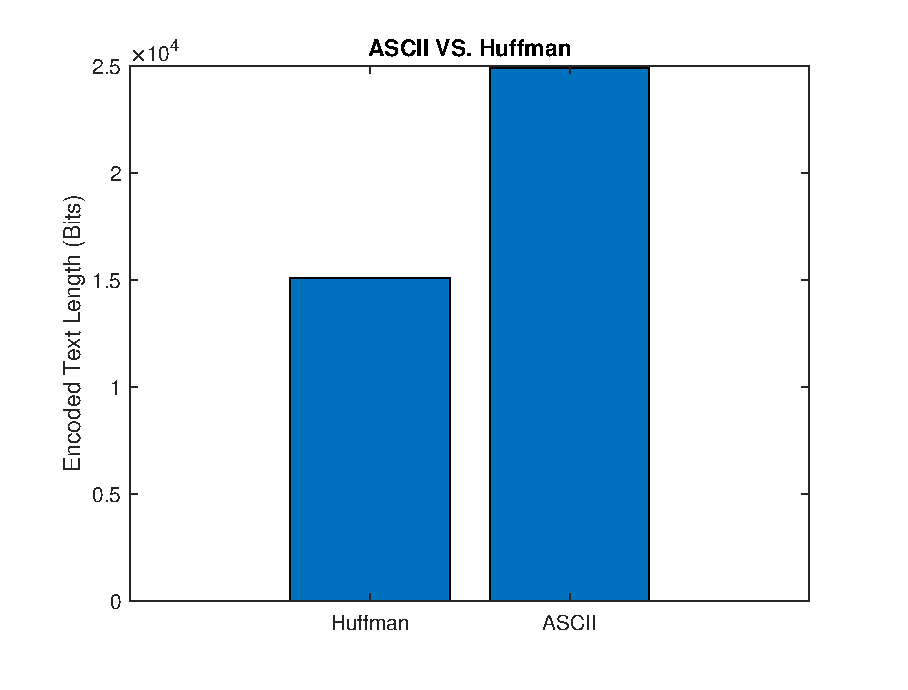
\includegraphics[width=\maxwidth{56.196688409433015em}]{figure_0.eps}
\end{center}

\begin{par}
\begin{flushleft}
We can now calculate the compression ratio by applying the formula:
\end{flushleft}
\end{par}

\begin{par}
$$\frac{\textrm{Length}\;\textrm{of}\;\textrm{Huffman}\;\textrm{code}}{\textrm{Length}\;\textrm{of}\;\textrm{ASCII}\;\textrm{code}}\times 100%$$
\end{par}

\begin{matlabcode}
% compRatio = ((asciiLen - huffLen)/asciiLen) * 100;
% fprintf("η = %f %%", compRatio)
compRatio = (huffLen / asciiLen) * 100;
fprintf("η = %f %%", compRatio)
\end{matlabcode}
\begin{matlaboutput}
η = 60.657055 %
\end{matlaboutput}


\matlabheading{Decoding}

\begin{par}
\begin{flushleft}
We now decode both the ASCII and the Huffman files to check for errors. We expect none due to the one-to-one mapping in both ASCII and Huffman:
\end{flushleft}
\end{par}

\begin{matlabcode}
decodedHuff = char(huffmandeco(encoded, dict));
decodedASCII = zeros(1, asciiLen);

for i = 1:7:asciiLen-6
    % We need to decode each 7 bits into a single character
    
    letterBits = extractBetween(ascii, i, i+6);
    
    letter = char(bin2dec(letterBits));
    if letter == ' '
        decodedASCII = strcat(decodedASCII," ");
    else
        decodedASCII = strcat(decodedASCII, letter);
    end
    
end
\end{matlabcode}
\begin{matlaboutput}
Warning: Input should be a string, character array, or cell array of character arrays.
\end{matlaboutput}
\begin{matlabcode}

decodeTable = cell2table({decodedASCII; decodedHuff});
decodeTable.Properties.VariableNames = {'Decoded File'};
decodeTable.Properties.RowNames = {'ASCII', 'Huffman'};
disp(decodeTable);
\end{matlabcode}
\begin{matlaboutput}
                                                                                                                                                                                                                                                                                                                                                                                                                                                                                                                                                                                                                                                                                                                                                                                                                                                                                                                                                                                                                                                                                                                                                                                                                                                                                                                                                                                                                                                                                                                                                                                                                                                                                                                                                                                                                                                            Decoded File                                                                                                                                                                                                                                                                                                                                                                                                                                                                                                                                                                                                                                                                                                                                                                                                                                                                                                                                                                                                                                                                                                                                                                                                                                                                                                                                                                                                                                                                                                                                                                                                                                                                                                                                                                                                                                              
               _______________________________________________________________________________________________________________________________________________________________________________________________________________________________________________________________________________________________________________________________________________________________________________________________________________________________________________________________________________________________________________________________________________________________________________________________________________________________________________________________________________________________________________________________________________________________________________________________________________________________________________________________________________________________________________________________________________________________________________________________________________________________________________________________________________________________________________________________________________________________________________________________________________________________________________________________________________________________________________________________________________________________________________________________________________________________________________________________________________________________________________________________________________________________________________________________________________________________________________________________________________________________________________________________________________________________________________________________________________________________________________________________________________________________________________________________________________________________________________________________________________________________________________________________________________________________________________________________________________________________________________________________________________________________________________________________________________________________________________________________________________________________________________________________________________________________________________________________________________________________________________________________________________________________________________________________________________________________________________________________________________________________________________________________________________________________________________________________________________________________________________________________________________________________________________________________________________________________________________________________________________________________________________________________________________________________________________________________________________________________________________________________________________________________________________________________________________________________________________________________________________________________________________________________________________________________________________________________________________________________________________________________________________________________________________________________________________________________________________________________________________________________________

    ASCII      "Lorem ipsum dolor sit amet, consectetur adipiscing elit. Pellentesque congue gravida leo, at euismod ligula fringilla vitae. Proin lobortis eleifend vestibulum. Donec eu vulputate velit. Donec vehicula quam nec tellus semper, at sollicitudin ex suscipit. Cras nisi nunc, porttitor sit amet tortor non, placerat dictum lorem. Maecenas volutpat metus in malesuada fringilla. Maecenas pulvinar eros in tempus eleifend. Phasellus vel rutrum ligula, ac porta massa. Vestibulum convallis, tellus non mollis luctus, arcu dolor fermentum purus, eget semper quam eros nec lacus. Maecenas consectetur, velit ac vestibulum facilisis, dolor ex ullamcorper diam, a tristique quam lorem sed metus. Nam blandit augue nunc, vitae mattis erat condimentum facilisis. Nullam porttitor, tortor accumsan lacinia efficitur, ex augue posuere nunc, a ultricies neque lorem quis arcu. Aliquam tempor enim quis suscipit porttitor. In hac habitasse platea dictumst. Mauris vehicula at justo vitae venenatis.Proin interdum porttitor nisl, blandit tristique nisl semper ut. Nullam vestibulum vitae justo nec pulvinar. Donec vitae consequat velit. Phasellus pharetra sapien ut egestas gravida. Sed ut semper ex. In dui erat, cursus in diam sit amet, placerat mollis lacus. Nunc fringilla blandit odio, non efficitur diam lacinia vitae. Cras a est pellentesque, rhoncus metus vitae, pulvinar eros. Aenean at tempus nulla. Maecenas sodales fermentum magna sit amet aliquet. Suspendisse ut diam sapien.Vestibulum in neque pharetra, auctor tellus pharetra, pharetra nisl. Fusce quis nisi scelerisque, congue augue quis, molestie mi. Pellentesque ligula lacus, commodo ut molestie ac, pretium sit amet magna. Curabitur varius sollicitudin leo quis aliquam. Mauris aliquam dictum elementum. Donec aliquet mi sem, rhoncus sagittis diam sodales non. Fusce facilisis pharetra augue sit amet auctor. Duis efficitur egestas velit hendrerit consectetur. Praesent eleifend porta est, at mattis urna bibendum eget. Nunc ultricies lorem eget nunc cursus, eget placerat diam dignissim. Nulla consequat lectus quis nisi consectetur lacinia. Integer efficitur lectus eu nisl rutrum, in ultricies mauris venenatis. Fusce in elit pretium, porta libero vitae, accumsan tortor. Proin nec est sed quam accumsan hendrerit eget eu augue. Donec lobortis convallis mi varius volutpat. Cras imperdiet malesuada risus.Nullam hendrerit porttitor enim, ac viverra odio pharetra sit amet. Fusce fringilla vitae nulla sed fermentum. Quisque varius commodo erat, vel vulputate libero rutrum et. Cras vehicula placerat orci, sagittis malesuada nulla tempor vulputate. Maecenas cursus ante mattis metus bibendum ullamcorper. Proin mauris augue, ultricies id odio vitae, fermentum elementum diam. Proin malesuada luctus nisl, ac sagittis erat pellentesque consectetur. Nam elementum velit non nisl tincidunt, finibus auctor eros interdum. Vivamus faucibus, enim sed placerat sagittis, diam tortor semper est, eget commodo sapien ligula eu diam. Phasellus eu ipsum eu metus pretium porta. Donec a tincidunt felis, sit amet accumsan sem. Nulla malesuada augue sed lectus venenatis, quis tincidunt orci consectetur. Integer faucibus a sem in pretium.Phasellus suscipit sapien dolor, ac ornare lorem tincidunt vitae. Maecenas tincidunt tempus urna, quis tincidunt velit viverra quis. Quisque vel elit lorem. Quisque vulputate, odio sit amet rhoncus condimentum, quam mi porta magna, in fermentum turpis enim in lorem. Fusce ullamcorper ut diam et iaculis. Sed lacinia vehicula tortor. Proin vel egestas turpis, vel blandit arcu."
    Huffman    "Lorem ipsum dolor sit amet, consectetur adipiscing elit. Pellentesque congue gravida leo, at euismod ligula fringilla vitae. Proin lobortis eleifend vestibulum. Donec eu vulputate velit. Donec vehicula quam nec tellus semper, at sollicitudin ex suscipit. Cras nisi nunc, porttitor sit amet tortor non, placerat dictum lorem. Maecenas volutpat metus in malesuada fringilla. Maecenas pulvinar eros in tempus eleifend. Phasellus vel rutrum ligula, ac porta massa. Vestibulum convallis, tellus non mollis luctus, arcu dolor fermentum purus, eget semper quam eros nec lacus. Maecenas consectetur, velit ac vestibulum facilisis, dolor ex ullamcorper diam, a tristique quam lorem sed metus. Nam blandit augue nunc, vitae mattis erat condimentum facilisis. Nullam porttitor, tortor accumsan lacinia efficitur, ex augue posuere nunc, a ultricies neque lorem quis arcu. Aliquam tempor enim quis suscipit porttitor. In hac habitasse platea dictumst. Mauris vehicula at justo vitae venenatis.Proin interdum porttitor nisl, blandit tristique nisl semper ut. Nullam vestibulum vitae justo nec pulvinar. Donec vitae consequat velit. Phasellus pharetra sapien ut egestas gravida. Sed ut semper ex. In dui erat, cursus in diam sit amet, placerat mollis lacus. Nunc fringilla blandit odio, non efficitur diam lacinia vitae. Cras a est pellentesque, rhoncus metus vitae, pulvinar eros. Aenean at tempus nulla. Maecenas sodales fermentum magna sit amet aliquet. Suspendisse ut diam sapien.Vestibulum in neque pharetra, auctor tellus pharetra, pharetra nisl. Fusce quis nisi scelerisque, congue augue quis, molestie mi. Pellentesque ligula lacus, commodo ut molestie ac, pretium sit amet magna. Curabitur varius sollicitudin leo quis aliquam. Mauris aliquam dictum elementum. Donec aliquet mi sem, rhoncus sagittis diam sodales non. Fusce facilisis pharetra augue sit amet auctor. Duis efficitur egestas velit hendrerit consectetur. Praesent eleifend porta est, at mattis urna bibendum eget. Nunc ultricies lorem eget nunc cursus, eget placerat diam dignissim. Nulla consequat lectus quis nisi consectetur lacinia. Integer efficitur lectus eu nisl rutrum, in ultricies mauris venenatis. Fusce in elit pretium, porta libero vitae, accumsan tortor. Proin nec est sed quam accumsan hendrerit eget eu augue. Donec lobortis convallis mi varius volutpat. Cras imperdiet malesuada risus.Nullam hendrerit porttitor enim, ac viverra odio pharetra sit amet. Fusce fringilla vitae nulla sed fermentum. Quisque varius commodo erat, vel vulputate libero rutrum et. Cras vehicula placerat orci, sagittis malesuada nulla tempor vulputate. Maecenas cursus ante mattis metus bibendum ullamcorper. Proin mauris augue, ultricies id odio vitae, fermentum elementum diam. Proin malesuada luctus nisl, ac sagittis erat pellentesque consectetur. Nam elementum velit non nisl tincidunt, finibus auctor eros interdum. Vivamus faucibus, enim sed placerat sagittis, diam tortor semper est, eget commodo sapien ligula eu diam. Phasellus eu ipsum eu metus pretium porta. Donec a tincidunt felis, sit amet accumsan sem. Nulla malesuada augue sed lectus venenatis, quis tincidunt orci consectetur. Integer faucibus a sem in pretium.Phasellus suscipit sapien dolor, ac ornare lorem tincidunt vitae. Maecenas tincidunt tempus urna, quis tincidunt velit viverra quis. Quisque vel elit lorem. Quisque vulputate, odio sit amet rhoncus condimentum, quam mi porta magna, in fermentum turpis enim in lorem. Fusce ullamcorper ut diam et iaculis. Sed lacinia vehicula tortor. Proin vel egestas turpis, vel blandit arcu."
\end{matlaboutput}
\begin{matlabcode}

% And now, we compare the decoded text with the original text:

if(strcmp(decodedHuff, originalText))
    disp("Huffman codes are error free as expected.")
end
\end{matlabcode}
\begin{matlaboutput}
Huffman codes are error free as expected.
\end{matlaboutput}
\begin{matlabcode}

if(strcmp(decodedASCII, originalText))
    disp("ASCII codes are error free as expected.")
end
\end{matlabcode}
\begin{matlaboutput}
ASCII codes are error free as expected.
\end{matlaboutput}


\begin{par}
\begin{flushleft}
We now output the Huffman decoded file for further inspection:
\end{flushleft}
\end{par}

\begin{matlabcode}
 
fid = fopen(strcat(path,"huffman.txt"),'w+');
\end{matlabcode}
\begin{matlaboutput}
Error using string/strcat (line 37)
Inputs must be character vectors, cell arrays of character vectors, or string arrays.
\end{matlaboutput}
\begin{matlabcode}
fprintf(fid, decodedHuff);
fclose(fid);
\end{matlabcode}

\matlabheading{Comments}

\begin{itemize}
\setlength{\itemsep}{-1ex}
   \item{\begin{flushleft} Huffman coding is a lossless coding method, which by definition means it's error free. \end{flushleft}}
   \item{\begin{flushleft} ASCII codes are made for computers to represent text, not for compression. We have 64 characters in our character list, which means we need only $\log_2 \left(64\right)=6\;\textrm{Bits}$ to represent each charachter, not $7\;\textrm{Bits}$. \end{flushleft}}
\end{itemize}


\matlabheading{Functions}

\begin{matlabcode}
function  [uniqueChars, pmfCharArr] = PMF(text)
            % Returns the probability of each charachter in an array
            
            textLen = length(text);
            uniqueChars = unique(text);
            uniques = length(uniqueChars);
            pmfCharArr = zeros(1, uniques);
            
            for idx = 1:uniques
                pmfCharArr(idx) = sum(text == uniqueChars(idx)) / textLen ;
            end
end
\end{matlabcode}

\end{document}
